\documentclass[11pt,a4paper]{article}
\usepackage[margin=2.3cm]{geometry}
\usepackage{fontspec}
\setmainfont{Times New Roman}
\usepackage{graphicx,booktabs,amsmath,amssymb,array,caption,float,xcolor,hyperref,microtype,needspace,adjustbox}
\usepackage[english]{babel}
\setlength{\emergencystretch}{2em}
\hypersetup{colorlinks=true,linkcolor=blue!50!black,citecolor=blue!50!black,urlcolor=blue!50!black}
\captionsetup{font=small,labelfont=bf}
\setlength{\parskip}{4pt}\setlength{\parindent}{0pt}
\title{SOAD: Observation-Aware Citrus Detection with Cross-View Aggregation and Quality Calibration}
\author{Author information to be added}
\date{}
\begin{document}
\maketitle

\begin{abstract}
Dense citrus detection is an essential perception task for autonomous robotic harvesting. Small fruit size, occlusion between adjacent instances, and similar background appearance make accurate localization and false-positive control challenging. We propose a \textbf{Sampling-Operator-Aware Detector (SOAD)} that integrates preservation of input observations, cross-tile instance aggregation, and candidate quality estimation into a complete detection pipeline. Overlapping tiles at the native pixel scale are used for both training and inference, allowing local fruit contours and appearance details to enter the RT-DETR-L network. Boundary filtering, coordinate restoration, and full-image deduplication then produce instance predictions. Complementary predictions from mirrored views are fused to refine object locations, while candidate evidence is used to estimate detection correctness and localization quality separately and obtain calibrated detection scores. The calibrators are fitted independently on the validation set, with the detector weights held fixed. On a held-out orchard and under comparable training iteration budgets, the complete SOAD pipeline improves mAP50:95 by 33.3\% relative to the full-image RT-DETR-L baseline and reduces false positives per image by 77.2\% at a recall of 0.70. The method improves small-fruit detection in dense scenes and background rejection at high recall, providing visual perception support for fruit localization, count estimation, and harvesting target selection.
\end{abstract}
\textbf{Keywords:} citrus detection; small objects; native-resolution tiling; RGB-D; confidence calibration; fruit counting

\section{Introduction}
Citrus detection and counting for robotic harvesting \cite{agyolo,mfaf,geosphere}, which aims at locating individual fruits and estimating their number in outdoor images, is a fundamental problem in agricultural robot perception. This problem is inherently ill-posed since leaf occlusion, overlapping fruits, and backgrounds with similar colors can cause different fruit boundaries or instance arrangements to produce similar two-dimensional observations; a single image does not always admit a unique solution. Existing methods typically constrain the solution space using priors on color, context, shape, or depth geometry. Beyond laboratory image analysis, autonomous harvesting requires perception outputs to reach the robot control system promptly. Camera resolution, edge computing capacity, and energy consumption are constrained in field deployment, precluding unrestricted increases in acquisition and inference resolution. The limited pixel support of small fruits is therefore a basic condition that detection and counting must address.

GeoSphere-DETR \cite{geosphere} is one of the representative methods that exploit geometric priors for citrus detection. It resizes RGB images and depth data to the network input scale, extracts multiscale visual features and curvature cues separately, predicts candidate boxes through geometric gating, and adjusts their scores using geometric consistency before counting. The RT-DETR family \cite{rtdetr,rtdetrv2} focuses on feature encoding and query selection, whereas AG-YOLO \cite{agyolo} and MFAF-YOLO \cite{mfaf} enhance orchard features and fusion across scales. These improvements operate after input sampling, and their effectiveness remains constrained by the discriminative fruit details retained in the network input. SAHI \cite{sahi} and ASAHI \cite{asahi} have demonstrated the benefits of slicing for small-object detection. In orchard RGB-D imagery, however, the visual information preserved by slicing changes how much additional information geometric cues can provide. When boundaries between adjacent fruits, or differences between fruits and yellow leaves, are compressed into a few pixels, improvements in box ranking must be examined separately from score changes introduced by geometric fusion.

Input resizing changes how well the network can distinguish fruit contours, gaps between adjacent instances, and differences from the background. Differences erased by sampling cannot be uniquely recovered by subsequent RGB feature encoding, so input organization directly affects the instance representations that the detector can learn. Depth geometry provides an additional observation, whose benefit depends on the information retained in the RGB input and the quality of geometric alignment. We organize training and inference around tiles at the native pixel scale, generate instance predictions through cross-tile assignment and full-image aggregation, and evaluate geometric fusion and decision calibration under matched input conditions.

We name the proposed pipeline the \textbf{Sampling-Operator-Aware Detector (SOAD)}. SOAD generates overlapping tiles that retain the pixel scale of the sensor image and assigns training annotations according to the intersection area between objects and tiles, maintaining a consistent input scale during training and inference. The detector predicts fruits within each tile, removes truncated boxes near internal tile boundaries, maps the remaining candidates to full-image coordinates, and removes duplicates. Predictions from the original and mirrored images are fused in a common coordinate system to reduce localization variability. Estimates of detection correctness and box localization quality are then used to adjust candidate scores. On the held-out orchard, the complete pipeline achieves a relative mAP50:95 improvement of 33.3\% over the full-image baseline.

\Needspace{10\baselineskip}
Overall, the contributions of this study are mainly in three aspects.
\begin{enumerate}
\item We establish a conditional analysis framework linking the \emph{observation operator, object representation, and geometric gain}. Sensor images, deterministic sampling, and detection decisions are represented as a sequence of information transformations. The ordering of optimal statistical risks characterizes the irreversible constraints imposed by input sampling, while effective object support on feature maps connects local discrimination, box localization, and instance separation. Within the same framework, the potential benefit of depth is defined as a conditional risk difference given the sampled RGB observation, rather than assuming that multimodal fusion is necessarily beneficial.
\item We develop SOAD, a sampling-operator-aware pipeline for citrus instance detection. Overlapping tiles at the native pixel scale form the detector inputs. During training, annotations are assigned by object intersection area and the proportion of empty tiles is controlled. During inference, internal-boundary filtering, coordinate remapping, and full-image deduplication maintain instance consistency across tiles. Candidate boxes from mirrored views are subsequently fused to reduce localization variability in local predictions.
\item We formulate a decomposed calibration loss for detection correctness and localization quality. Fruit-matching labels and matched IoU targets are constructed for candidate boxes. Binary log loss trains the true-fruit probability estimator, squared loss trains quality regression, and the two predictions are combined using a weight selected on the validation set. The loss is applied to post-detection calibration models so that scores reflect both instance correctness and localization quality. Feature ablations assess the contribution of evidence such as depth and curvature.
\end{enumerate}

Input sampling determines the visual evidence available to subsequent representations and affects the conditional benefit of depth geometry. The following sections review related methods, describe SOAD, and present experimental results, including the performance contribution and computational cost of each stage.

\section{Related Work}
\subsection{Real-Time Detection and Citrus Detection in Orchards}
Real-time object detection balances accuracy and computational cost through feature encoding, query matching, and bounding-box regression. RT-DETR \cite{rtdetr} achieves end-to-end detection using an efficient hybrid encoder and IoU-aware query selection, while RT-DETRv2 \cite{rtdetrv2} further improves multiscale sampling and training strategies. D-FINE (2025) \cite{dfine} formulates box regression as a probability distribution refined across layers and improves regression quality through localization self-distillation. DEIM \cite{deim} strengthens one-to-one matching supervision by increasing the number of objects per training image and uses a matching-aware loss to improve optimization for samples of different quality. These methods improve representation efficiency, localization accuracy, and supervision utilization, respectively. Their internal network optimization nevertheless depends on object information already retained in the input and cannot directly compensate for instance differences removed by full-image resizing before feature extraction. To address this input constraint, \textbf{SOAD} uses native-pixel tiles as the common observation unit for training and inference and reconstructs complete detection outputs through full-image instance aggregation.

Orchard detectors adapt general-purpose networks to foliage occlusion, illumination changes, and variations in fruit size. AG-YOLO \cite{agyolo} and MFAF-YOLO \cite{mfaf} enhance fruit features through global context and adaptive multiscale fusion, respectively. YOLO-MECD (2025) \cite{mecd} targets both on-tree and fallen fruits, combining efficient multiscale attention, partial convolution modules, and MPDIoU loss to improve detection while reducing model size. ACDNet (2026) \cite{acdnet} incorporates fruit-aware feature extraction, dynamic multiscale sampling, and shape-aware IoU loss to adapt sampling locations and localization supervision to citrus morphology. These methods address small fruits and occlusion, but their feature sampling and shape constraints still act on the observations received by the network. Adding attention or shape priors does not automatically eliminate contour and inter-instance gap losses caused by input compression. \textbf{SOAD} therefore preserves the local pixel scale before feature learning and handles truncated instances through area-based annotation assignment and internal-boundary filtering, accounting for both input detail and instance integrity.

Recent studies also address detail degradation caused by feature downsampling. SCORE-DETR (2025) \cite{scoredetr} introduces a frequency aggregation network and a Haar wavelet fusion module for small and occluded citrus fruits, enhancing object signals and alleviating aliasing during multiscale fusion. FG-DETR (2026) \cite{fgdetr} combines dynamic feature encoding, spatial and frequency-domain enhancement, and wavelet downsampling to retain high-frequency details while suppressing complex background responses. These studies establish detail preservation as an important topic in orchard detection. They preserve feature information already present within the network, whereas object differences removed by resizing before network entry remain beyond the scope of these mechanisms. \textbf{SOAD} moves detail preservation to the observation stage, using native-pixel tiles to reduce additional input compression and relating observation operators to detection risk to explain the implications for subsequent feature learning.

\subsection{Small-Object Slicing and Cross-View Instance Aggregation}
Sliced detection decomposes large images into local inputs, increasing the effective spatial extent of small objects at a fixed network input size. SAHI \cite{sahi} combines overlapping sliced inference with slicing-aided fine-tuning, addressing both local inputs and training adaptation. The ASAHI preprint (2026) \cite{asahi} adapts the number of slices to image resolution, combines full-image and sliced training samples, and uses Cluster-DIoU-NMS to handle duplicate detections, with particular emphasis on reducing redundant computation caused by a fixed slice size. Slicing and deduplication improve the visible object scale. In overlapping regions of dense fruit scenes, however, repeated observations of the same instance coexist with overlap between different instances. Aggregation based only on geometric box similarity still faces difficulties in assigning truncated boxes and distinguishing neighboring instances. \textbf{SOAD} assigns training labels according to object intersection area and filters truncated candidates near internal tile boundaries before coordinate remapping and full-image deduplication, maintaining instance assignment rules from local learning to full-image output.

Cross-view fusion uses multiple predictions of the same instance to reduce localization variability. Weighted boxes fusion \cite{wbf} combines coordinates of same-class candidates according to confidence, providing a general approach to exploiting localization information from multiple predictions. ASAHI \cite{asahi} instead uses center distance and overlap to suppress duplicate boxes. These approaches emphasize coordinate integration and duplicate removal, respectively, and both require reliable instance matching in dense detection. Geometric aggregation alone does not model candidate correctness; false boxes on similar backgrounds may also receive high scores or exhibit consistency across views. \textbf{SOAD} therefore separates mirror box fusion from evidence calibration, first integrating localization information in a common coordinate system and then adjusting final scores using candidate context and box-related evidence.

\subsection{RGB-D Fusion and Conditional Geometric Gains}
RGB-D fruit detection exploits the complementarity of color texture and spatial structure to reduce appearance ambiguity. GeoSphere-DETR (2026) \cite{geosphere} derives curvature cues from depth, selects geometric features through learnable spatial gating, and introduces geometry-consistency rescoring at the candidate level. This method explicitly addresses depth reliability and false positives on similar backgrounds, allowing geometry to participate in both representation learning and output decisions. Modeling geometric reliability does not, however, directly establish the conditional contribution of an additional observation relative to existing RGB evidence. As the degree of RGB input compression changes, the discriminative information supplied by the same geometric cue also changes. \textbf{SOAD} incorporates input sampling into detection risk analysis and constructs an independent control using RGB--geometry tiles with synchronized cropping and augmentation, examining the additional role of geometry after local visual evidence is preserved.

The source of geometric representations also affects the interpretation of fusion results. CIAFNet (2026) \cite{ciafnet} uses cross-modal interaction, adaptive fusion, and multiscale aggregation with pseudo-depth generated by Depth Anything V2 in natural orchards, and further adapts to measured sensor depth in controlled scenes. Pseudo-depth infers structural priors from the same RGB image, whereas measured depth comes from an additional sensor observation. They differ in information source, missing-data patterns, and noise distributions. Such fusion mechanisms address the selection and adaptation of structural representations. Interpreting the learning benefits of these representations directly as independent sensor information gains would nevertheless conflate representation priors, observation quality, and input scale. \textbf{SOAD} distinguishes RGB observation organization from additional geometric evidence and analyzes geometric gains with tile scale and spatial correspondence held consistent, linking modality contributions to detection input conditions.

\subsection{Calibration of Detection Correctness and Localization Quality}
Detection confidence supports both candidate ranking and threshold-based selection, but class scores do not necessarily agree with bounding-box localization quality. Bridging Precision and Confidence \cite{bpc} introduces a calibration loss during detector training to reduce the discrepancy between confidence and detection correctness. In work published online in 2026, Lee et al.\ \cite{trackcal} use tracked boxes in video as temporally consistent localization references and an IoU-aware weighted loss to mitigate tracking noise in annotation-free post-calibration. These approaches depend on calibration constraints during detector training or temporal references in video, respectively. Neither directly replaces candidate quality estimation after cross-tile and mirror aggregation for independent orchard images. With the detector frozen, \textbf{SOAD} uses validation-set matching correctness and matched IoU to supervise classification and quality regression separately, yielding a decomposed calibration objective for full-image aggregated outputs.

For fruit false positives, geometric rescoring in GeoSphere-DETR \cite{geosphere} turns shape consistency into a criterion for candidate selection, whereas tracking-assisted calibration \cite{trackcal} constructs quality references from temporal consistency. These methods show that score adjustment depends on whether auxiliary evidence agrees with actual detection quality, rather than merely changing the score range. A single geometric or temporal consistency cue remains subject to missing depth, local occlusion, and correspondence errors, and cannot fully characterize the distinction between candidate correctness and localization quality in independent still images. \textbf{SOAD} combines detection scores, within-image context, and box-related descriptors as candidate evidence. It learns correctness and localization quality separately for rescoring and examines the contribution of each evidence group through feature removal and false-positive analysis at fixed recall.

\section{Method}
\subsection{Overall Framework}
SOAD generates native-pixel tiles from RGB images, uses tiles at the same scale for training and inference, and restores local detections to full-image instances. Mirror fusion and evidence rescoring operate on the detector outputs. To measure the conditional benefit of geometric cues, a separate GeoSphere-DETR control receives synchronized RGB and B/N curvature maps. Figure~\ref{fig:pipe} shows the placement of these operations during training and inference.

\begin{figure}[H]
\centering
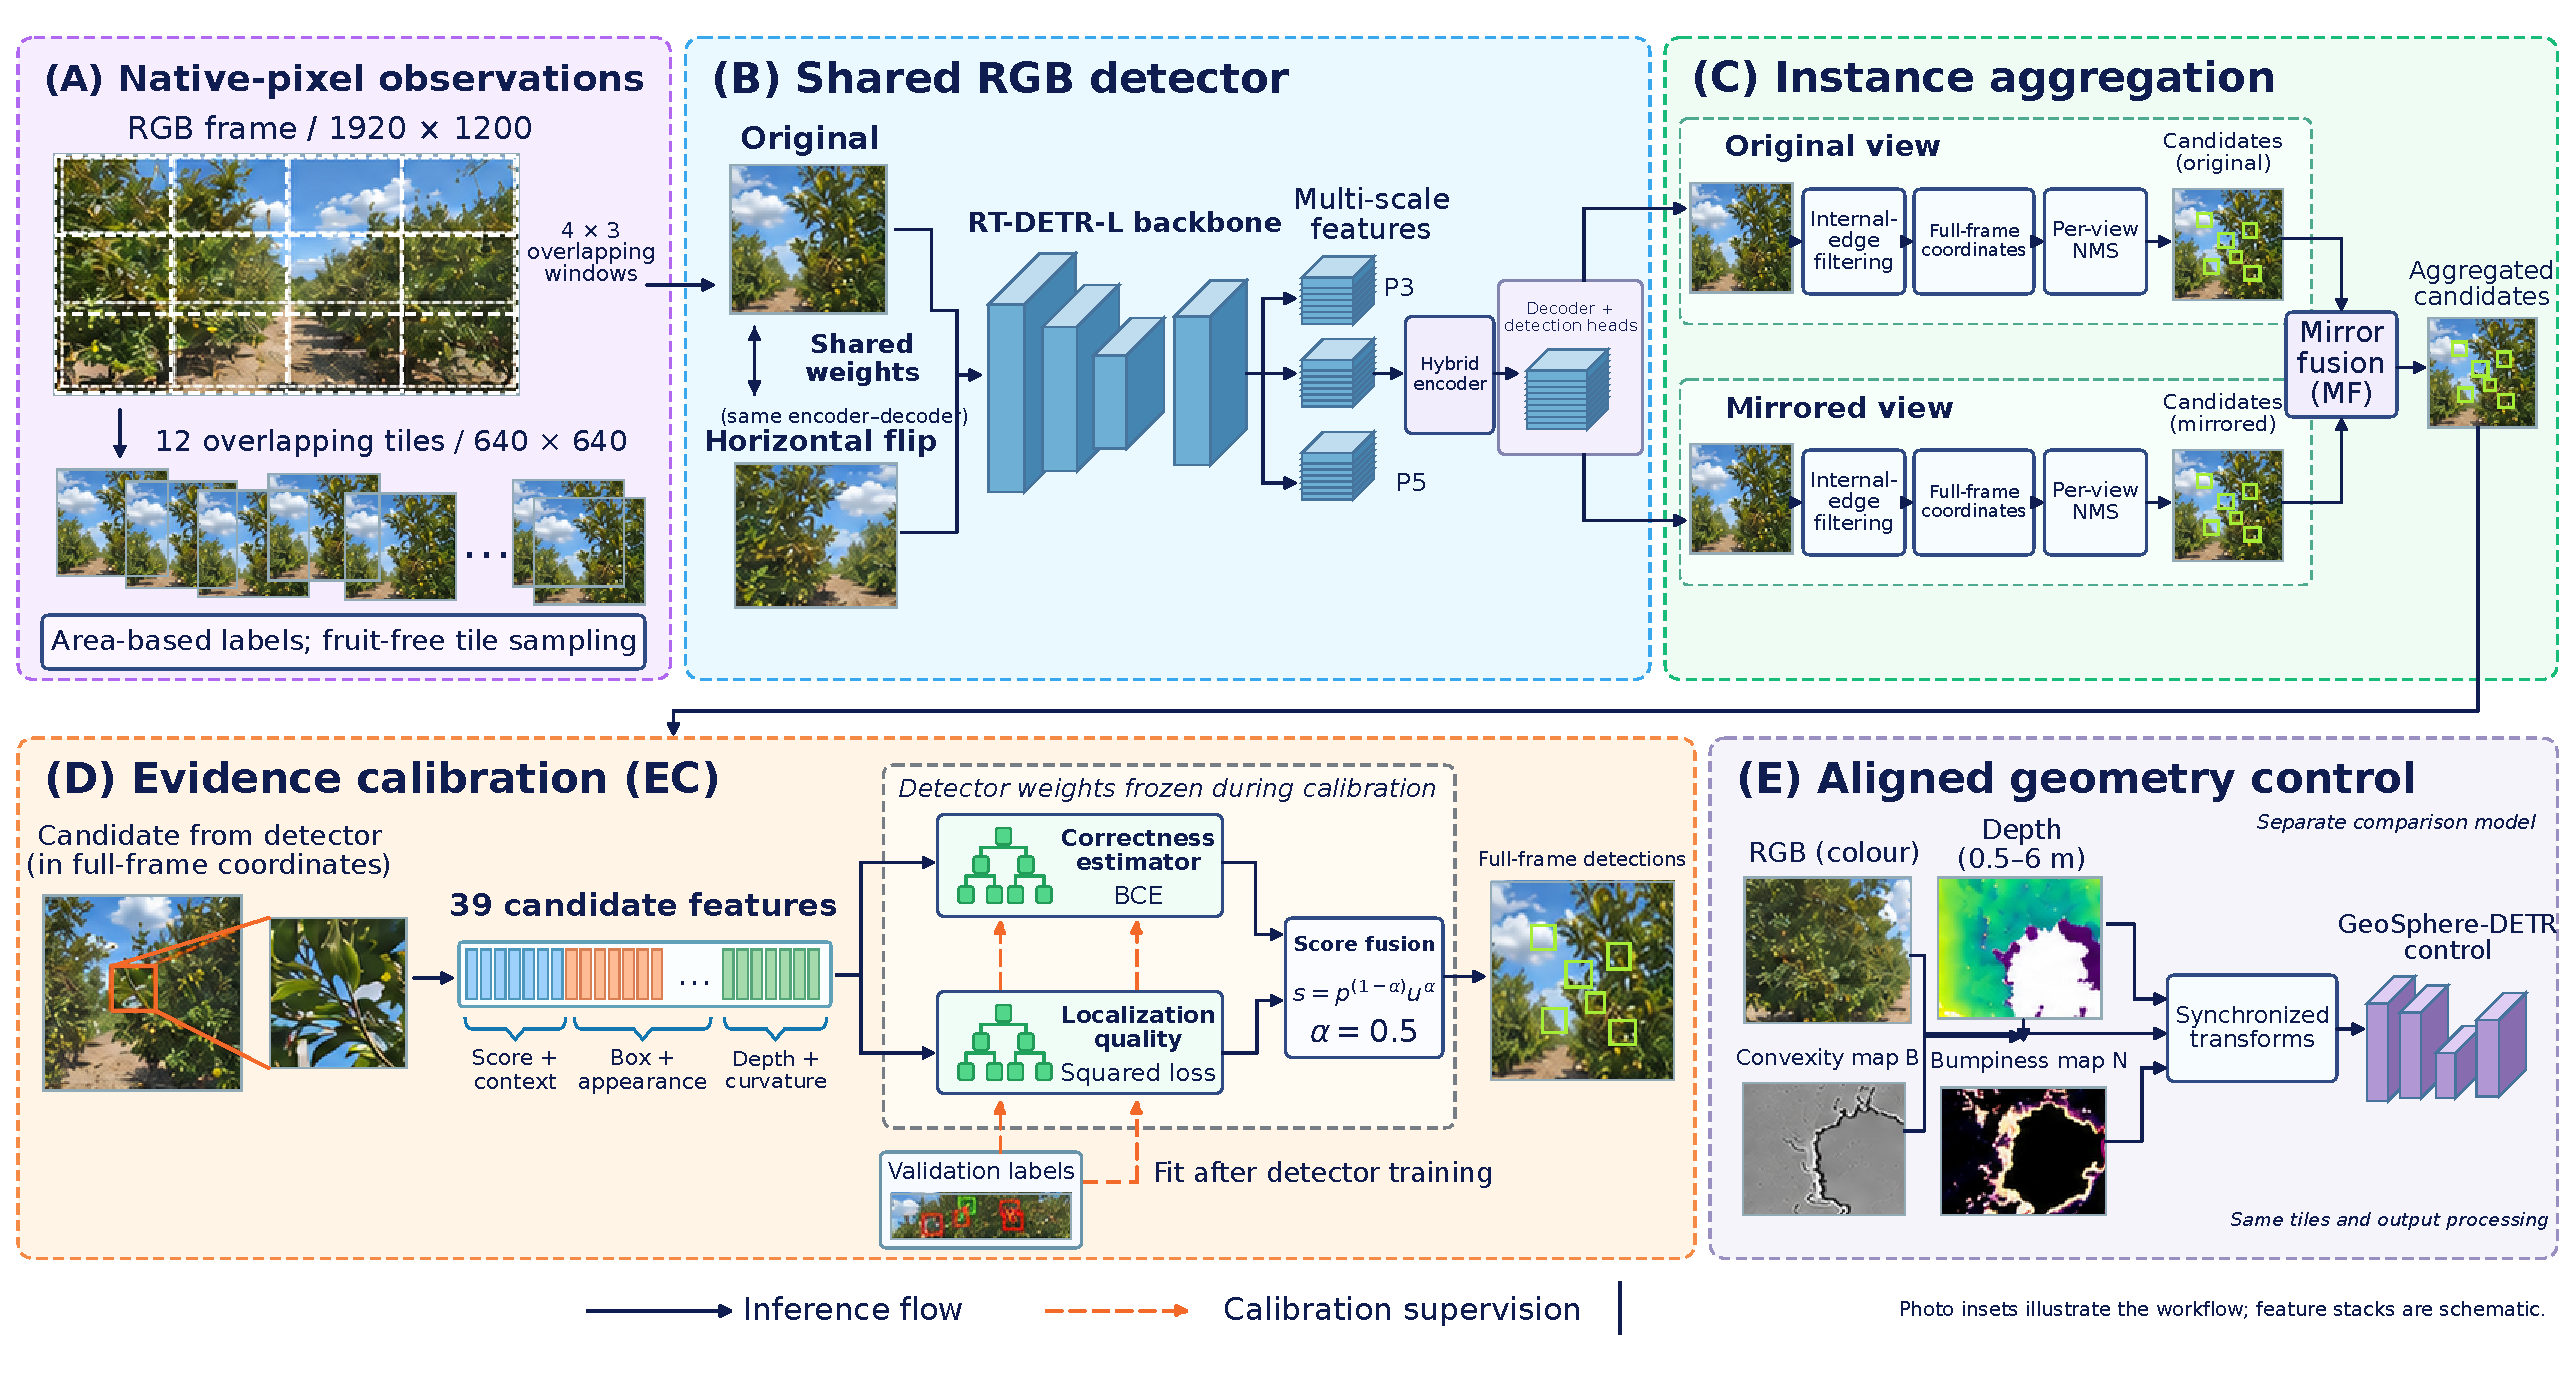
\includegraphics[width=0.98\linewidth]{../figures/fig_pipeline.pdf}
\caption{Overall framework of \textbf{SOAD}. (A) Native-pixel overlapping tiles and training annotation organization. (B) The original and mirrored views share the RT-DETR-L detection network. (C) Boundary filtering, coordinate restoration, and deduplication are performed per view, followed by mirror fusion (MF). (D) Candidate evidence is used to estimate detection correctness and localization quality separately, which are combined into calibrated scores (EC). The calibrators are fitted independently using validation-set supervision while the detector weights remain fixed. (E) An independent geometric control with synchronized RGB and B/N curvature inputs, separate from the main detection network.}
\label{fig:pipe}
\end{figure}
Figure~\ref{fig:pipe} organizes SOAD into three stages: preserving local observations, restoring instance coordinates, and adjusting candidate quality. Overlapping tiles provide local inputs at the native pixel scale. Coordinate remapping and full-image deduplication convert local predictions into a countable instance set, while mirror fusion and evidence calibration further refine localization and selection. This structure connects input organization to instance outputs in a complete detection pipeline, clarifies dependencies between the method components, and provides the structural basis for the subsequent ablations.

\subsection{Observation Operators and Detection Risk}
\label{sec:observation}
Let $I\in\mathbb{R}^{H\times W\times3}$ denote the sensor RGB image, $Y$ the annotations consisting of fruit classes and bounding boxes, and $G\in\mathbb{R}^{H\times W\times2}$ optional geometry maps derived from depth. Given a detection or counting loss $\ell$, define the optimal statistical risk for any observation $Z$, without restricting model capacity, as
\begin{equation}
\mathcal{R}^{*}(Z)=\inf_{f}\mathbb{E}\!\left[\ell\bigl(f(Z),Y\bigr)\right].
\end{equation}
Let $D_S$ be a deterministic operator that resizes the full image to network width $S$. Every decision based on $D_S(I)$ can be simulated by a model receiving the complete image that first computes $D_S$ and then applies the same decision rule. Therefore,
\begin{equation}
\mathcal{R}^{*}(I)\leq\mathcal{R}^{*}\!\bigl(D_S(I)\bigr).
\label{eq:risk}
\end{equation}
Equation~\eqref{eq:risk} characterizes the information ordering between complete and resized observations when the capacity of the decision function is unrestricted, providing a theoretical basis for retaining local details already captured by the camera. Actual gains for finite-capacity detectors are assessed through training and evaluation. The theoretical conditional gain from adding geometry is $\Delta_G^{*}(D_S)=\mathcal{R}^{*}(D_S(I))-\mathcal{R}^{*}(D_S(I),G)\geq0$, whose magnitude depends on the input operator and the information quality of $G$. We therefore measure geometric model gains under identical tiling and synchronized alignment, connecting the theoretical information gain to actual model performance.

Detector feature maps translate the effect of the input operator into spatial support. If a fruit has width $w$ in the sensor image, the input transformation has scale factor $\alpha$, and feature level $\ell$ has stride $q_\ell$, its approximate extent on that feature map is $\rho_\ell=\alpha w/q_\ell$. This is not a threshold for successful detection, but it shows that object representation, box localization, and separation of neighboring instances within the same network change with the sampling operator. Images in this dataset are 1920 pixels wide, giving $\alpha\approx1/3$ for a full-image input width of 640 pixels. The median fruit box side length is 21.1 pixels, corresponding to approximately 7.0 input pixels. These values illustrate the scale in this dataset; the relation expressed by Eq.~\eqref{eq:risk} and $\rho_\ell$ does not depend on these particular values.

\subsection{Training on Native-Pixel Tiles}

Each 1920$\times$1200 image is divided into $4\times3$ tiles of 640$\times$640 pixels, with horizontal origins $\{0,\allowbreak 427,\allowbreak 853,\allowbreak 1280\}$ and vertical origins $\{0,\allowbreak 280,\allowbreak 560\}$. Adjacent tiles overlap by 213 or 280 pixels. An annotation is assigned to a tile only if its intersection with that tile covers at least half of the box area, after which it is clipped to the tile boundary. Training retains all fruit-containing tiles and one quarter of fruit-free tiles using a fixed random seed. Validation and testing use all twelve tiles per image. The 14,792 training tiles are obtained from 1,492 loadable training images and contain 184,642 tile-level boxes. With a batch size of 8, ten training epochs require approximately 18,490 iterations, close to the 18,700 iterations of one hundred full-image epochs. The model remains a COCO-pretrained RT-DETR-L, with its loss function and backbone unchanged.

\subsection{Tile Inference, Boundary Handling, and Full-Image Deduplication}
For tile origin $(x_t,y_t)$, a box in tile coordinates $b_t=(x_1,y_1,x_2,y_2)$ is mapped back to the full image by adding the origin. A detection is discarded if it lies within 2 pixels of an internal tile boundary; overlap allows neighboring tiles to observe the complete fruit. Retained boxes are deduplicated by class-specific non-maximum suppression with an IoU threshold of 0.5. Only the 300 highest-scoring boxes are retained, matching the output limit for a single full-image detection pass. This deterministic boundary rule avoids unstable coordinate averaging for truncated fruits.

\subsection{Mirror Fusion and Optional Score Calibration}
Each tile undergoes an additional horizontally mirrored inference pass, and the mirrored detections are mapped back to the original coordinates. Following weighted boxes fusion \cite{wbf}, same-class boxes are greedily clustered at an IoU threshold of 0.55. For cluster $\mathcal{C}$, coordinates are combined using the confidence-weighted mean
\begin{equation}
\bar b=\frac{\sum_{j\in\mathcal{C}}s_j b_j}{\sum_{j\in\mathcal{C}}s_j},
\qquad
\bar s=\frac{\sum_{j\in\mathcal{C}}s_j}{2}.
\end{equation}
The second expression normalizes over two views, assigning lower scores to boxes found in only one view. This step requires 24 rather than 12 network inference passes.

For detections with confidence above 0.02, the calibrator computes 39 candidate features describing scores and within-image context, box shape, depth and surrounding rings, physical size, curvature maps, and HSV color. Let $y_i\in\{0,1\}$ denote the fruit-matching label for candidate $i$ at IoU 0.5, and let $q_i$ be its maximum overlap with a same-class annotation. The classification model $p_\theta(x_i)$ estimates the probability of a true fruit, and the regression model $u_\phi(x_i)$ estimates the quality target $y_iq_i$. Two gradient-boosting models \cite{lgbm} minimize binary log loss and squared loss, respectively. Since their parameters are independent, training can be expressed as the decomposed calibration objective
\begin{equation}
\mathcal{L}_{\mathrm{cal}}=\sum_i\ell_{\mathrm{BCE}}\!\left(y_i,p_\theta(x_i)\right)
+\sum_i\left(u_\phi(x_i)-y_iq_i\right)^2.
\label{eq:cal_loss}
\end{equation}
The calibrated score combines the two predictions with exponential weights,
\begin{equation}
s_{\mathrm{cal}}=\hat p^{1-\alpha}\hat u^{\alpha},\qquad \alpha=0.5.
\end{equation}
The models and $\alpha$ are selected only through five-fold out-of-fold predictions grouped by image on the validation set. The held-out orchard is never used for fitting. Equation~\eqref{eq:cal_loss} describes post-detection calibration training; this loss is not used to train the RT-DETR-L backbone. The contributions of depth and curvature features are evaluated by measuring performance differences after removing the corresponding features.

\subsection{Controlled Comparison with Aligned Geometry Inputs}
To assess whether geometric cues remain beneficial after preserving object scale, the B and N curvature maps are appended to RGB as the fourth and fifth channels. Mosaic, affine, and flip transforms are applied jointly to all five channels, while color perturbations affect RGB only. After augmentation, the geometry maps are separated and passed to the gated branch of the reference architecture. The compared RGB and geometric models thus share the same tiles, training epochs, inference protocol, and evaluation procedure. The geometry-gated branch serves as a controlled comparison and is not part of the main RGB pipeline.

\section{Experiments and Results}
\subsection{Dataset, Splits, and Evaluation Protocol}
We use the public RGB-D citrus dataset \cite{dataset,geosphere}, which contains 2,200 images and 102,719 annotated instances, divided into 1,500 training, 200 validation, and 500 test images. Test images were collected in a different orchard and on different dates. Each sample contains a 1920$\times$1200 RGB frame, a 16-bit depth map in millimeters, B/N curvature maps, and annotations for on-tree and ground fruits. This section examines the data and observation conditions, detection gains from tiled inputs, the role of the calibration objective, and the conditional benefit and computational cost of geometric inputs. All performance measures are computed in full-image coordinates.

\begin{table}[H]
\centering
\small
\caption{Splits and class distribution of the RGB-D citrus dataset.}
\label{tab:data}
\begin{adjustbox}{max width=\linewidth}
\begin{tabular}{lrrrr}
\toprule
Split & Images & On-tree fruits & Ground fruits & Total instances \\
\midrule
Training & 1,500 & 71,382 & 6,384 & 77,766 \\
Validation & 200 & 8,041 & 664 & 8,705 \\
Test & 500 & 14,780 & 1,468 & 16,248 \\
\midrule
Total & 2,200 & 94,203 & 8,516 & 102,719 \\
\bottomrule
\end{tabular}
\end{adjustbox}
\par\vspace{2pt}\parbox{0.97\linewidth}{\footnotesize Statistics refer to the original dataset splits. Eight training images and one test image with negative annotation coordinates are excluded. All models are evaluated on the same 499 test images containing 16,199 fruit instances.}
\end{table}
Table~\ref{tab:data} includes both on-tree and ground fruits, with an approximately $10:1$ instance ratio in the test set. The task therefore emphasizes dense canopy fruits while also accounting for fallen fruits. The independently held-out orchard tests transfer across scenes, and the common set of 499 valid images and 16,199 instances ensures that methods are compared on the same evaluation samples. This composition places SOAD's instance detection and full-image counting design under realistic class imbalance and provides an experimental basis for assessing transfer across orchards.
\begin{figure}[H]
\centering
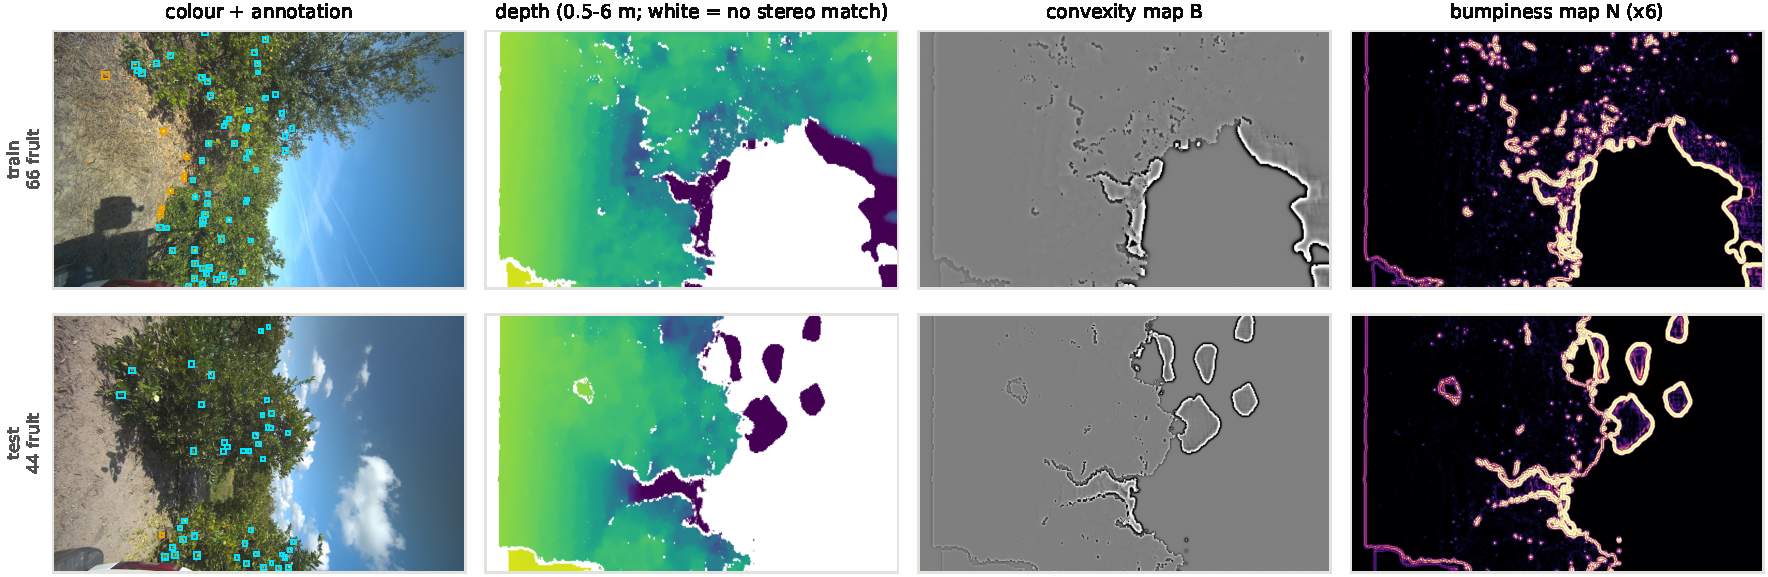
\includegraphics[width=0.98\linewidth]{../figures/fig_data_modalities.pdf}
\caption{Complex appearance and incomplete geometry jointly challenge orchard detection. Examples from the training and held-out orchards show RGB, depth, and B/N curvature maps, where B denotes convexity and N denotes bumpiness. The stored images are rotated by 90 degrees.}
\label{fig:mod}
\end{figure}
Figure~\ref{fig:mod} illustrates the task conditions motivating the preservation of local visual evidence in SOAD. Foliage and fruits have similar colors, making visible edges and inter-instance gaps important discriminative cues in occluded regions. Missing depth and curvature responses on foliage also cause the utility of geometry to vary spatially. Native-pixel tiles retain these visible details in the detector input, and the geometric control evaluates the contribution of additional observations. These scene characteristics support organizing local RGB inputs before assessing supplementary geometric information.
\begin{figure}[H]
\centering
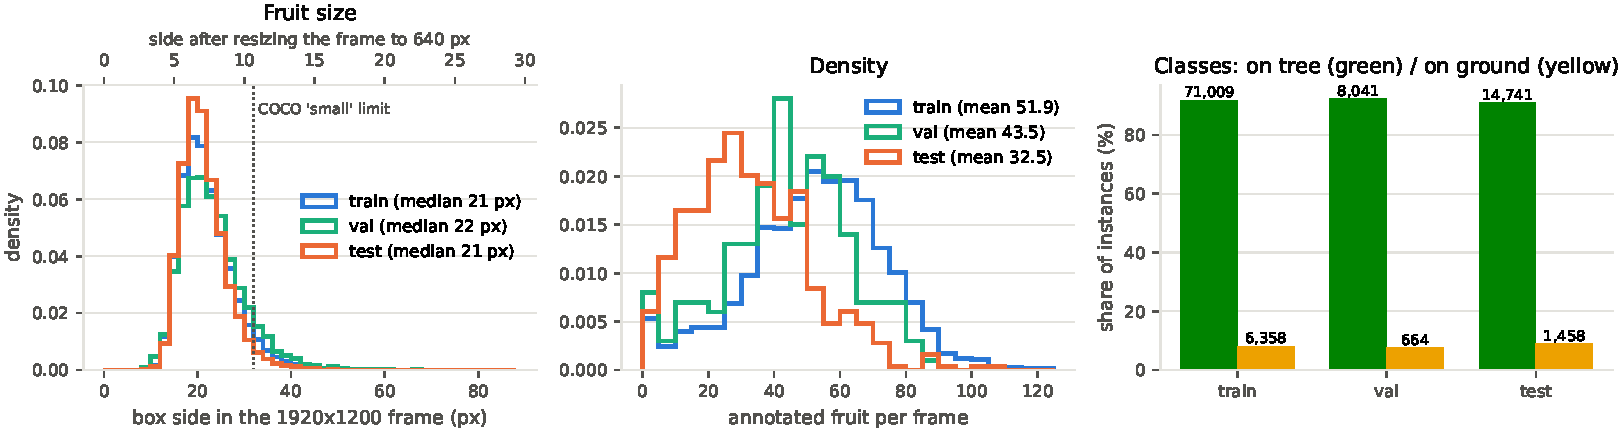
\includegraphics[width=0.98\linewidth]{../figures/fig_data_size_density.pdf}
\caption{Small object size and dense instances make full-image resizing further compress the available observations. Fruit size, density, and class proportions are shown for each split, together with the corresponding object sizes after resizing the full image to a width of 640 pixels.}
\label{fig:size}
\end{figure}
Figure~\ref{fig:size} relates the need for input organization to object scale and instance density. The median fruit side length is approximately 21--22 pixels across the splits, and training images contain an average of 51.9 fruits. Reducing the image width to one third leaves a median object side length of approximately 7 pixels and a box area of approximately one ninth of the original. Both individual fruit appearance and gaps between neighboring instances are compressed, making the preservation of local sampling an important design consideration for dense detection. This distribution motivates SOAD's native-pixel tiling, whose practical benefit is further assessed through size-specific recall and full-image detection results.
\begin{figure}[H]
\centering
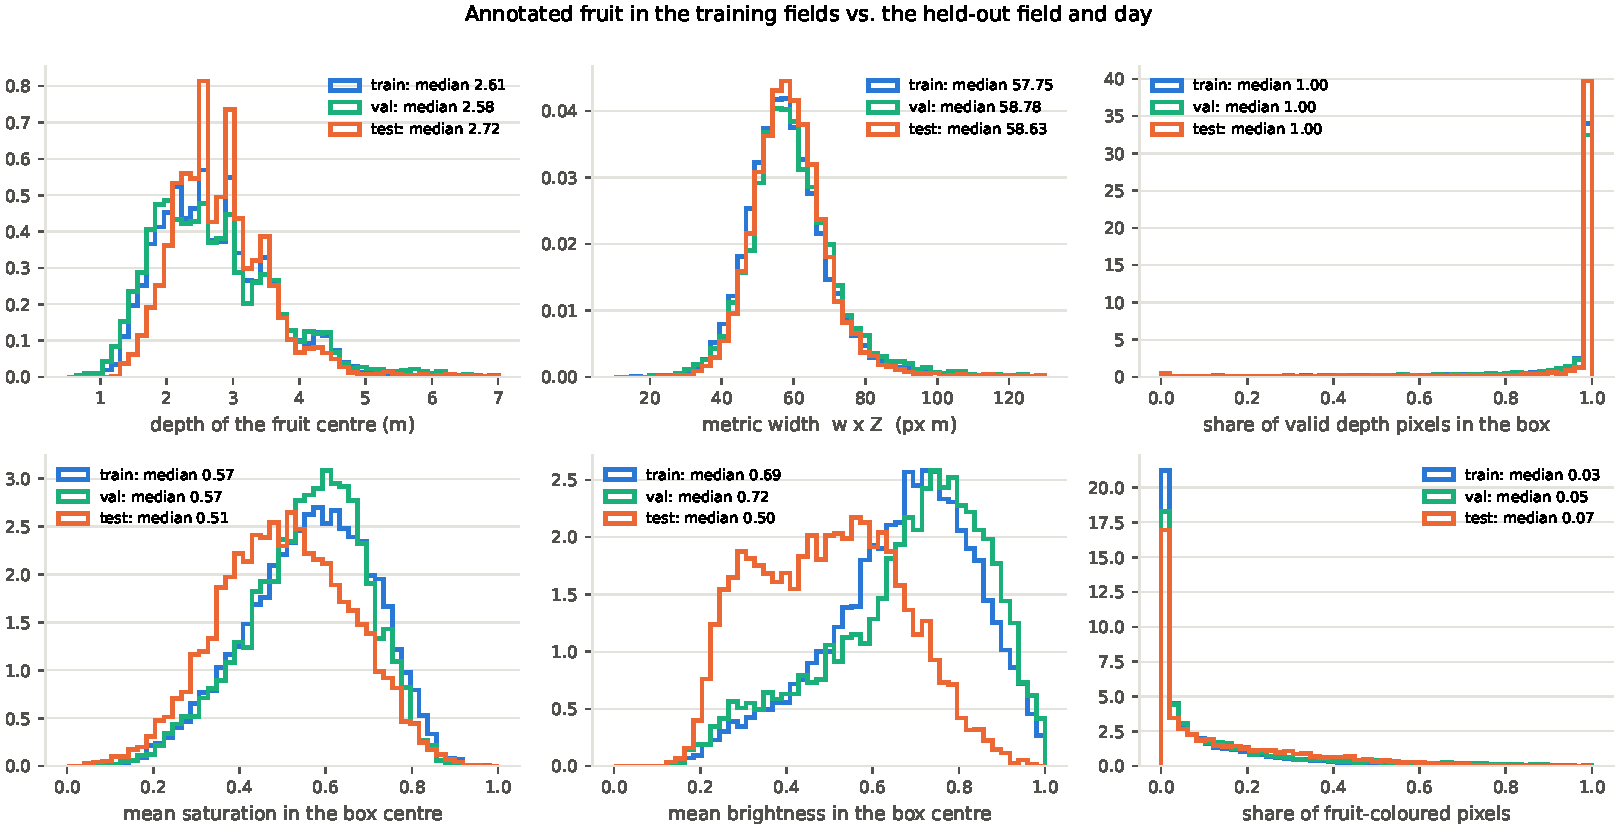
\includegraphics[width=0.98\linewidth]{../figures/fig_data_domain_shift.pdf}
\caption{The held-out orchard has scale proxies similar to the training set but different color statistics. Center depth, width multiplied by depth, valid-depth fraction, and color distributions are compared. The scale proxy is expressed in pixel-meters and is not converted to actual physical width.}
\label{fig:shift}
\end{figure}
Figure~\ref{fig:shift} shows that the held-out orchard introduces additional appearance variation. The median width-times-depth scale proxy changes from 57.75 to 58.63 pixel-meters, a relative difference of approximately 1.5\%, whereas median brightness changes from 0.69 to 0.50 and saturation from 0.57 to 0.51. Similar scale proxies and different color statistics jointly test local structure recognition and candidate selection across scenes. Together with the subsequent gains in held-out accuracy and counting, these data conditions provide an evaluation basis for SOAD's local input organization and evidence calibration across orchards.

All models use the same offline evaluator, applying the matching and AP rules of the public implementation in full-image coordinates. In addition to mAP50 and mAP50:95, we report recall and false positives per image (FPPI) at confidence 0.25 and IoU 0.5, as well as FPPI at recalls of 0.70 and 0.80. Per-image counting error is the mean absolute difference between detected and annotated fruit counts at confidence 0.25. Model and calibration parameters are selected using the validation set; the held-out orchard is used only for final evaluation. Statistical intervals are obtained from 1,000 paired resamples of images and reflect image-sampling variation rather than variation across training seeds.

\subsection{Input Alignment and Scale Diagnostics}
The effect of the geometric branch is interpretable only when RGB and curvature maps are aligned pixelwise. The alignment probe replaces each geometry map with the grayscale version of its RGB image. After identical geometric augmentation, the two inputs should retain high pixel correlation. Training budgets are compared in terms of network updates: ten tile-training epochs require approximately 18,490 updates, while one hundred full-image epochs require approximately 18,700.

\begin{figure}[H]
\centering
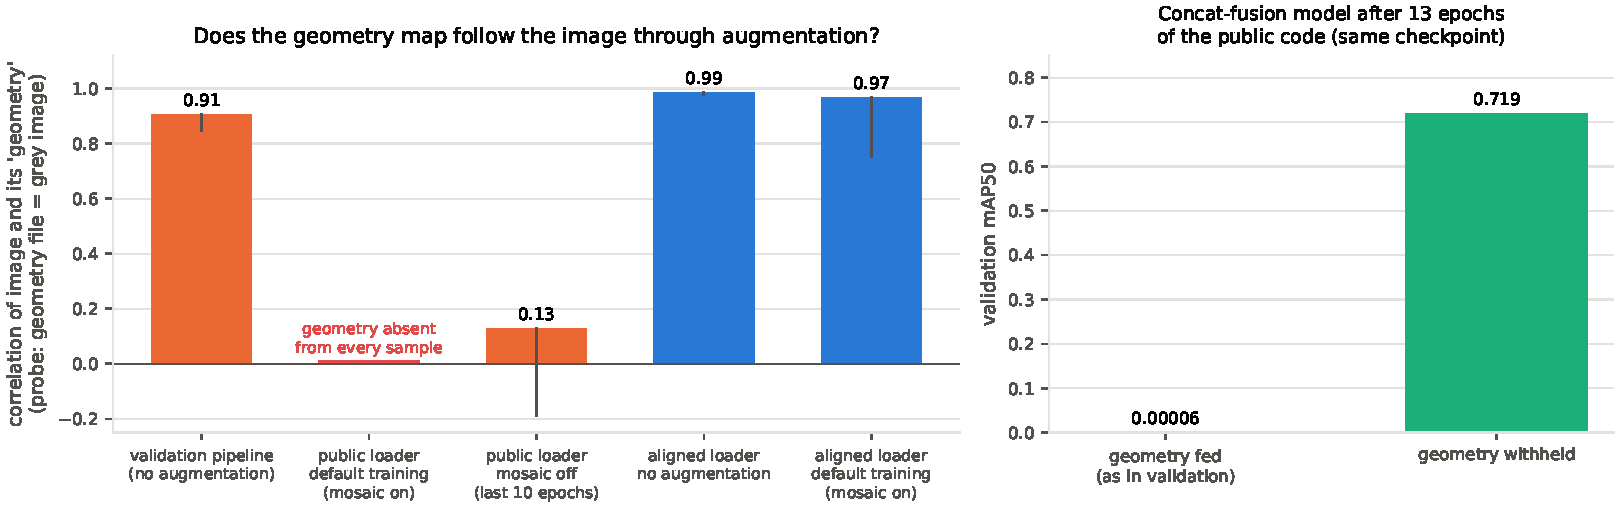
\includegraphics[width=0.98\linewidth]{../figures/fig_alignment.pdf}
\caption{Synchronized augmentation preserves spatial correspondence between modalities. Left: alignment probing with grayscale RGB substituted for geometry. Right: detection results from the same concatenation-fusion checkpoint with the anomalous geometry input retained or removed.}
\label{fig:align}
\end{figure}
Figure~\ref{fig:align} verifies that synchronized augmentation preserves spatial correspondence. The correlation between the grayscale probe and the RGB input increases from 0.13 to 0.97. In comparison, default separate loading loses the geometry input in all 40 inspected mosaic samples. Removing the anomalous geometry input from the concatenation-fusion model restores mAP50 from nearly zero to 0.719, further demonstrating that input organization directly affects the usable observations reaching fusion modules. Synchronized augmentation therefore provides a reliable input basis for conditional geometric analysis, ensuring that the geometric control has explicit pixel correspondence.
\begin{figure}[H]
\centering
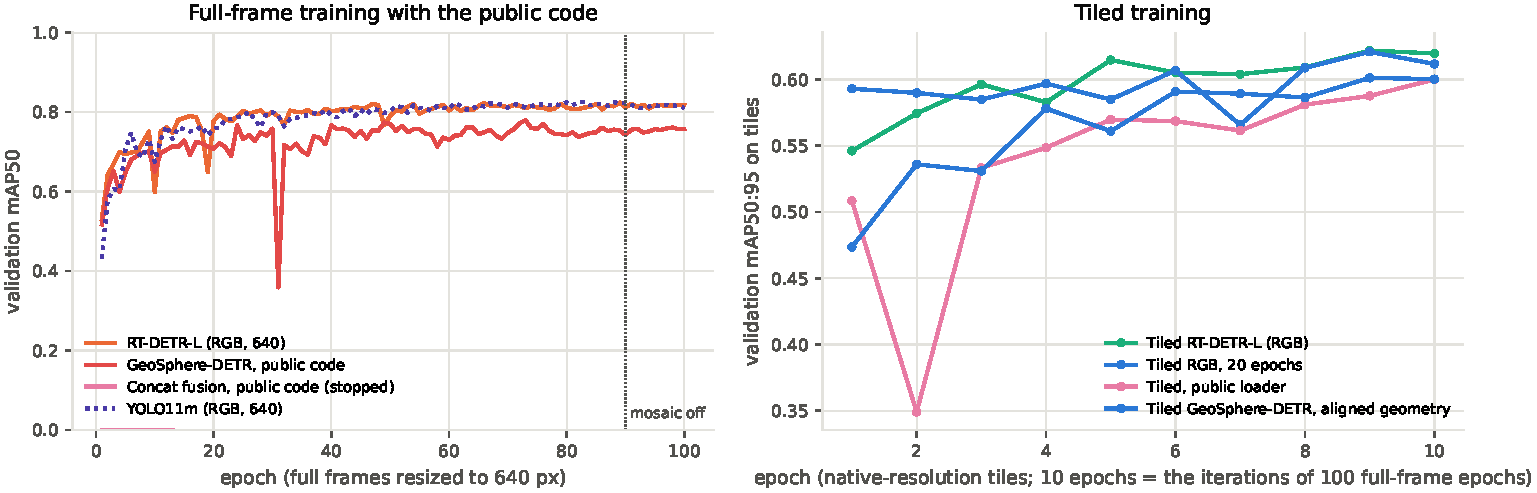
\includegraphics[width=0.98\linewidth]{../figures/fig_training_curves.pdf}
\caption{Full-image and tile-training trends under comparable update budgets. The left panel uses mAP50 and the right panel uses mAP50:95, so their curve heights are not directly comparable. Ten tile-training epochs and one hundred full-image epochs require similar numbers of updates.}
\label{fig:curves}
\end{figure}
Figure~\ref{fig:curves} shows SOAD's training progress under comparable parameter-update budgets. Full-image and tile training require approximately 18,700 and 18,490 updates, respectively, a difference of approximately 1.1\%. The curves describe the training trends of mAP50 and mAP50:95 separately; final accuracy is compared using the common metrics in Table~\ref{tab:main}. Under this budget, the tiled configuration achieves higher held-out accuracy, showing that allocating updates to local samples at the native pixel scale yields useful detection gains. This result supports incorporating input organization into SOAD's training design.

For this dataset, RT-DETR-L backbone, and training budget, tiled input provides the largest accuracy increment among the changes examined. It jointly changes object pixel scale, local context, training sample composition, and the number of inference passes, so the measured gain pertains to the complete input pipeline. Improvements in both detection accuracy and false positives at matched recall under comparable iteration budgets provide empirical support for designing the detection pipeline around observation organization.

\subsection{Main Detection Performance and False-Positive Operating Points}
Table~\ref{tab:main} compares SOAD with RT-DETR-L (2024) \cite{rtdetr}, YOLO11m (2024) \cite{yolo11}, and GeoSphere-DETR (2026) \cite{geosphere}, for which measurements under the same protocol are available. The RGB detection path of SOAD is selected using validation mAP50:95 after mirror fusion. SOAD component ablations are reported in Table~\ref{tab:configs}, and paired differences involving geometric models are given in Table~\ref{tab:geometry_stats}.

\begin{table}[H]
\centering
\scriptsize\setlength{\tabcolsep}{4pt}
\caption{Comparison of SOAD with recent methods evaluated in this study. All results use the same 499 images and 16,199 fruits from the held-out orchard and the same full-image evaluator.}
\label{tab:main}
\begin{adjustbox}{max width=\linewidth}
\begin{tabular}{lrrrrrrr}
\toprule
Method/configuration & mAP50$\uparrow$ & mAP50:95$\uparrow$ & FPPI$\downarrow$ & Recall$\uparrow$ & \shortstack{FPPI@\\R.70$\downarrow$} & \shortstack{FPPI@\\R.80$\downarrow$} & \shortstack{Count\\error$\downarrow$} \\
\midrule
RT-DETR-L (2024) \cite{rtdetr} & 0.697 & 0.432 & 53.17 & 0.843 & 9.57 & 23.66 & 48.8 \\
YOLO11m (2024) \cite{yolo11} & 0.640 & 0.391 & 12.44 & 0.690 & 13.69 & 37.97 & 5.7 \\
GeoSphere-DETR (2026) \cite{geosphere} & 0.677 & 0.419 & 23.50 & 0.790 & 9.53 & 26.19 & 16.8 \\
\midrule
\textbf{SOAD (12 passes)} & 0.813 & 0.566 & 7.60 & 0.844 & 2.35 & 5.32 & 4.5 \\
\textbf{Ours (SOAD, 24 passes)} & \textbf{0.824} & \textbf{0.576} & \textbf{7.37} & \textbf{0.946} & \textbf{2.18} & \textbf{5.24} & \textbf{4.4} \\
\bottomrule
\end{tabular}
\end{adjustbox}
\par\vspace{2pt}\parbox{0.97\linewidth}{\footnotesize Publication or release years and citations follow method names; YOLO11 cites its official release documentation. The first three rows use resized full-image inputs with one network pass per image. Pass counts in SOAD names refer to 640-pixel network inference passes per image. The 12-pass configuration retains evidence calibration and disables mirror fusion, corresponding to w/o MF in Table~\ref{tab:configs}; the 24-pass configuration is the complete SOAD selected on the validation set. Both SOAD configurations use tiled inputs. Bold indicates the best value in each performance column, and $\uparrow/\downarrow$ denotes higher/lower is better. FPPI, recall, and counting error use confidence 0.25; FPPI@R uses fixed recall.}
\end{table}
Table~\ref{tab:main} shows that combining input organization with output processing in SOAD improves both cross-orchard detection accuracy and false positives at matched recall. Compared with full-image RT-DETR-L, mAP50:95 increases by 14.4 percentage points, and FPPI@R.70 decreases from 9.57 to 2.18, a reduction of approximately 77.2\%. The paired mAP50:95 test gives $p<0.001$ (Table~\ref{tab:ladder}). This statistically significant accuracy gain supports the effectiveness of the complete SOAD pipeline. The two configurations require 1 and 24 inference passes, respectively, so their performance difference corresponds to different input and computational configurations.

In the control with matched tiles and additional output processing, SOAD has lower FPPI@R.70 and FPPI@R.80 than the geometric model, supporting background false-positive control at high recall. The geometric control achieves mAP50:95 of 0.580, compared with 0.576 for SOAD, and also has lower fixed-threshold FPPI and counting error. The interval for the mAP50:95 difference is $-0.001$ to $+0.009$, with $p=0.100$; see Table~\ref{tab:geometry_stats} and Fig.~\ref{fig:ladder}. These results distinguish the performance characteristics of the two approaches. Positive evidence for SOAD is concentrated in false positives at matched recall and overall gains over the full-image baseline. The main configuration is selected on the validation set, and statistical comparisons assess image-sampling differences with model weights fixed.

\begin{figure}[H]
\centering
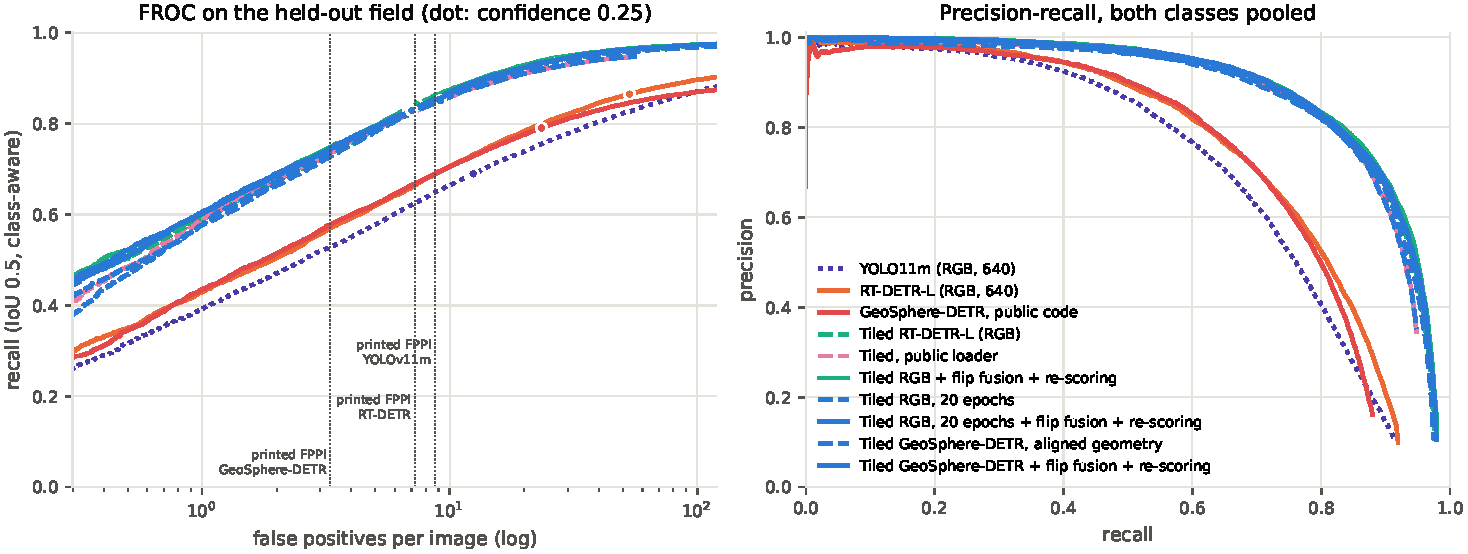
\includegraphics[width=0.98\linewidth]{../figures/fig_froc_pr.pdf}
\caption{Detection benefits of tiled input extend across confidence operating points. Circles on the FROC and precision--recall curves indicate confidence 0.25. Vertical lines for literature-reported false-positive rates are references only because their corresponding recall values are unavailable.}
\label{fig:froc}
\end{figure}
Figure~\ref{fig:froc} extends the improvement of SOAD over full-image baselines to multiple confidence operating points. The FROC curves of tiled models lie above those of full-image models over a broad false-positive range, indicating that more fruits can be detected for a given false-positive budget. The PR curves at high recall further demonstrate effective candidate selection. Curves remain similar before and after calibration while the fixed-threshold operating points move, showing that evidence calibration adjusts the set of retained candidates. Across continuous operating points, this result supports the complementary roles of input organization and output calibration, with benefits in both detection capability and output usability.

The geometric control further illustrates the role of evaluation at matched recall. At confidence 0.25, the tiled RGB and aligned geometric models have recalls of 0.943 and 0.851 and FPPI values of 30.87 and 9.18, respectively. At a fixed recall of 0.70, their FPPI values are 2.49 and 2.45. A common operating point separates false-positive control from the fraction of candidates retained, providing a clear basis for evaluating SOAD's calibration module. After mirror fusion, validation mAP50:95 is 0.643 for the RGB model and 0.639 for the geometric model, supporting the validation-based selection of the ten-epoch RGB detection path.

\begin{figure}[H]
\centering
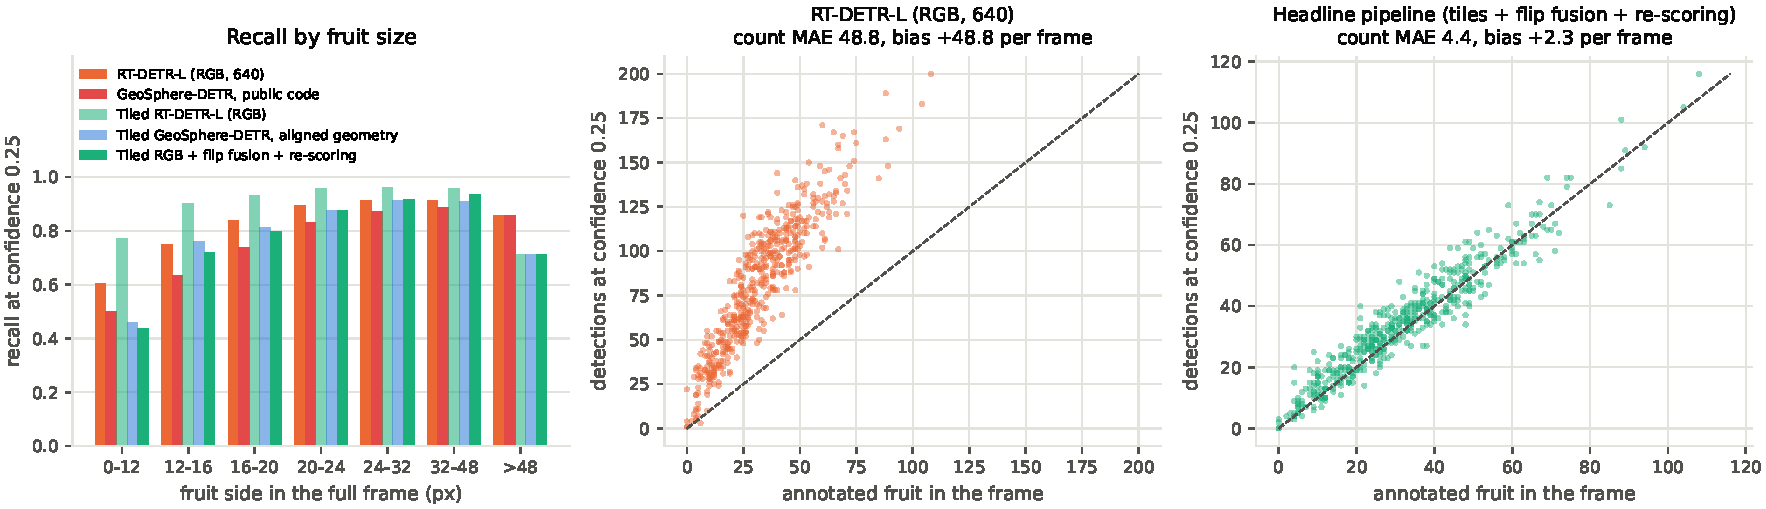
\includegraphics[width=0.98\linewidth]{../figures/fig_size_count.pdf}
\caption{Joint improvement in small-fruit detection and full-image counting. Left: size-specific recall at confidence 0.25. Center and right: predicted versus annotated counts for the full-image baseline and complete SOAD, respectively.}
\label{fig:count}
\end{figure}
Figure~\ref{fig:count} connects gains in small-fruit detection to full-image counting quality. The tiled RGB model achieves higher recall in most small-size groups, supporting the benefit of native-pixel inputs for difficult small objects. The predicted counts of complete SOAD are closer to the annotations: count mean absolute error decreases from 48.8 for the full-image baseline to 4.4, a reduction of approximately 91.0\%, and mean overcount bias decreases from 48.8 to 2.3. This result shows that preserving local inputs, aggregating full-image instances, and calibrating candidate evidence can jointly translate detection improvements into more accurate fruit counts, directly supporting SOAD's integrated detection and counting design.

\begin{figure}[H]
\centering
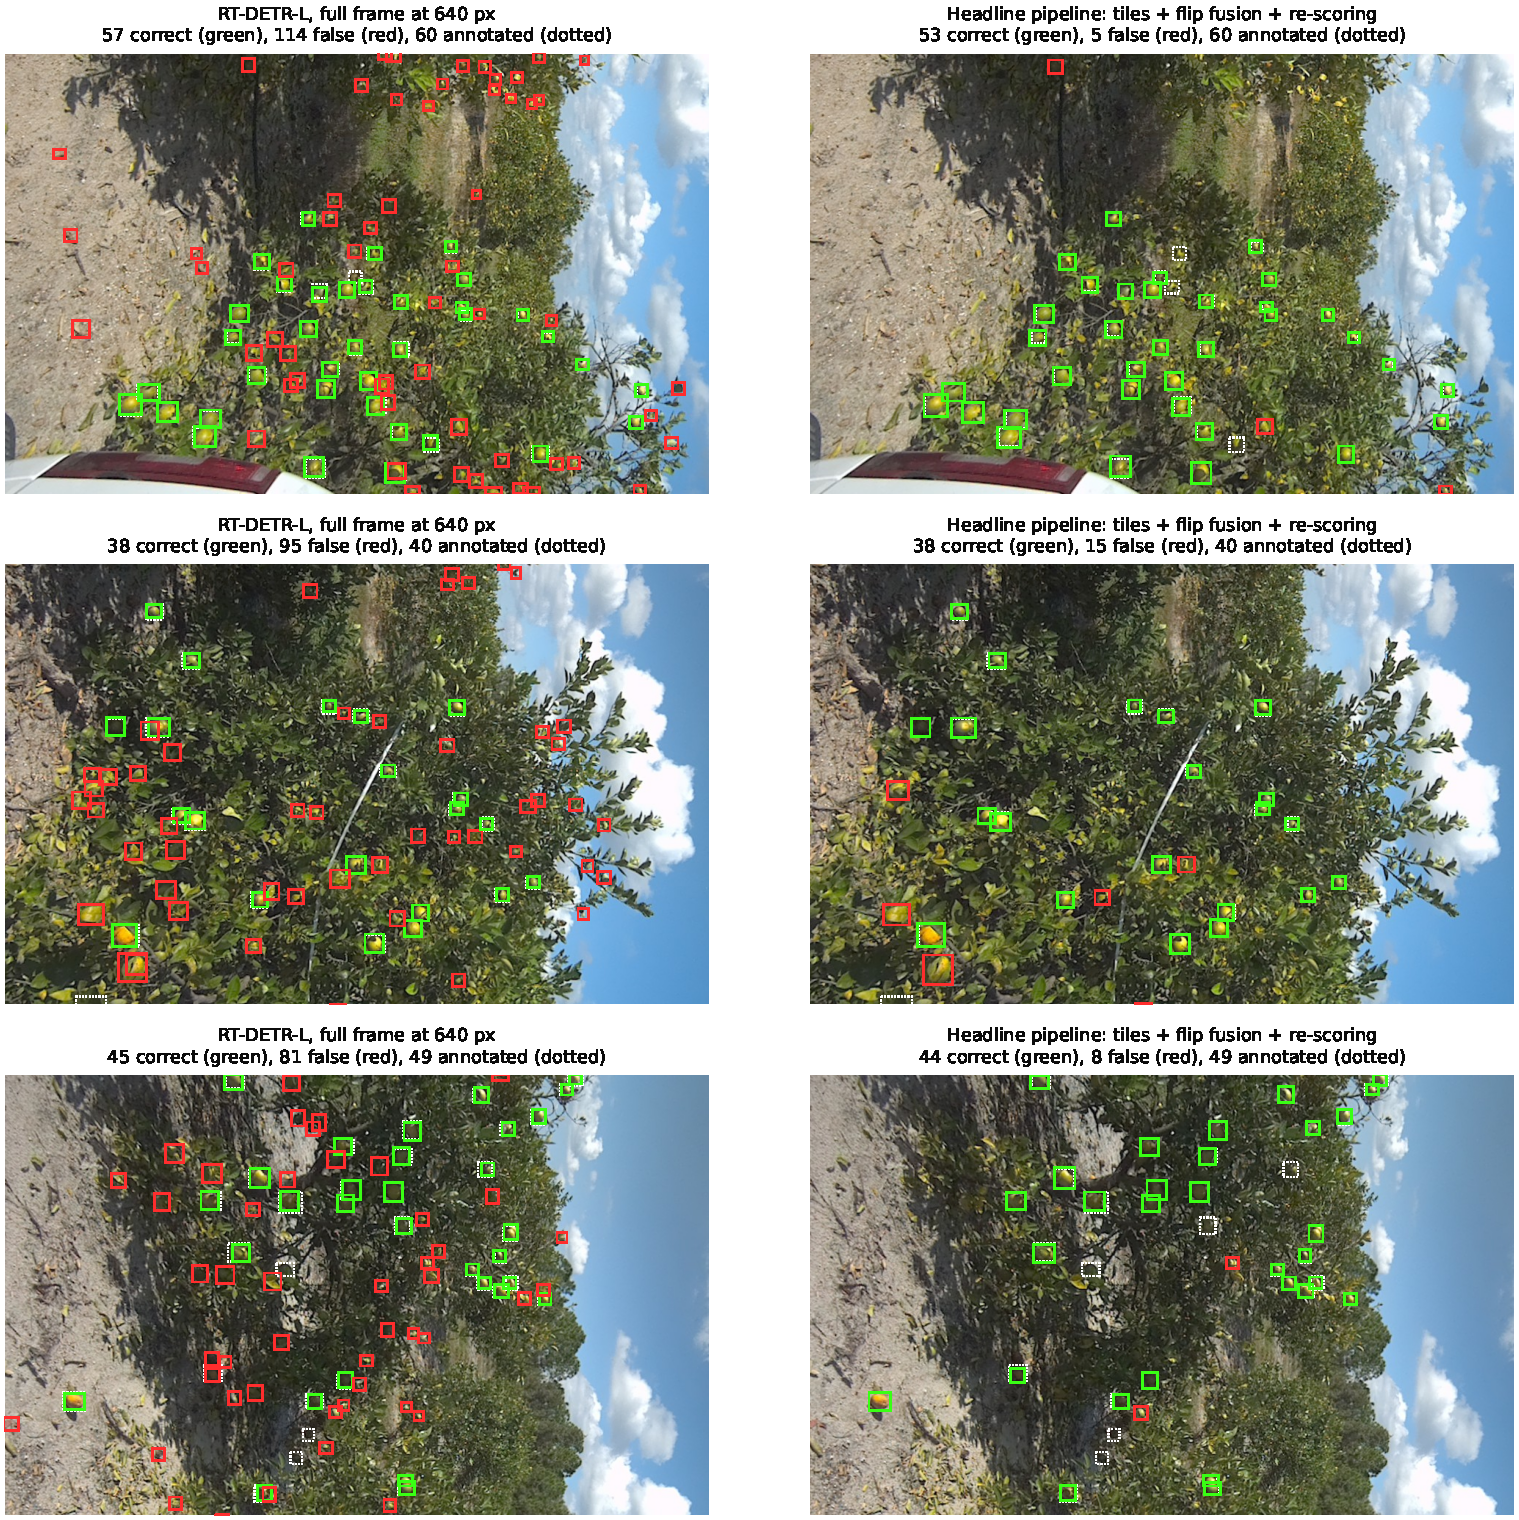
\includegraphics[width=0.98\linewidth]{../figures/fig_qualitative.pdf}
\caption{Complete SOAD substantially reduces false positives in the illustrated challenging backgrounds. Left: full-image RT-DETR-L. Right: SOAD. Green boxes indicate correct detections at IoU 0.5, red boxes indicate false positives, and dashed white boxes denote annotations.}
\label{fig:qual}
\end{figure}
Figure~\ref{fig:qual} illustrates SOAD's rejection of yellow leaves, bright soil, and reflective backgrounds. False positives decrease by approximately 95.6\%, 84.2\%, and 90.1\% in the three examples, while retaining approximately 93.0\%, 100\%, and 97.8\% of the baseline's correct detections, respectively. Substantial false-positive reductions with most correct detections retained show that the complete pipeline distinguishes the illustrated background responses from real fruits. These cases provide visual support for SOAD's candidate selection and are consistent with lower false positives at matched recall and improved counting across the full test set.

RT-DETR-L, YOLO11m, and GeoSphere-DETR serve as independently evaluated baselines, sharing the same data split, valid test samples, and full-image evaluator. Comparisons pertain to these three baselines and the input and computational configurations listed in Table~\ref{tab:main}.

\subsection{Component Contributions and Evidence Rescoring}
This section examines SOAD's input organization, mirror fusion, and evidence calibration. Table~\ref{tab:configs} defines SOAD variants by removing components; the geometric baseline comparison is included in Table~\ref{tab:main}.

\begin{table}[H]
\centering
\scriptsize\setlength{\tabcolsep}{4pt}
\caption{Ablation of SOAD output modules. All four configurations use the same ten-epoch checkpoint, native-pixel tiles, and cross-tile aggregation; only mirror fusion and evidence calibration are switched on or off.}
\label{tab:configs}
\begin{adjustbox}{max width=\linewidth}
\begin{tabular}{lrrrrrrrr}
\toprule
Variant & Passes & mAP50$\uparrow$ & mAP50:95$\uparrow$ & FPPI$\downarrow$ & Recall$\uparrow$ & \shortstack{FPPI@\\R.70$\downarrow$} & \shortstack{FPPI@\\R.80$\downarrow$} & \shortstack{Count\\error$\downarrow$} \\
\midrule
\textbf{SOAD} w/o MF \& EC & 12 & 0.812 & 0.567 & 30.87 & 0.943 & 2.49 & 5.29 & 29.0 \\
\textbf{SOAD} w/o MF & 12 & 0.813 & 0.566 & 7.60 & 0.844 & 2.35 & 5.32 & 4.5 \\
\textbf{SOAD} w/o EC & 24 & 0.819 & 0.574 & 29.22 & 0.865 & 2.35 & 5.27 & 27.5 \\
\midrule
\textbf{Ours (SOAD)} & 24 & \textbf{0.824} & \textbf{0.576} & \textbf{7.37} & \textbf{0.946} & \textbf{2.18} & \textbf{5.24} & \textbf{4.4} \\
\bottomrule
\end{tabular}
\end{adjustbox}
\par\vspace{2pt}\parbox{0.97\linewidth}{\footnotesize MF denotes mirror fusion and EC denotes evidence calibration; w/o indicates removal of the corresponding component. Bold indicates the best value in each performance column. Inference passes and metrics are defined as in Table~\ref{tab:main}.}
\end{table}
Table~\ref{tab:configs} provides direct ablation evidence for combining mirror fusion and evidence calibration. Mirror fusion increases the base configuration's mAP50:95 from 0.567 to 0.574. Adding calibration alone reduces counting error from 29.0 to 4.5, with mAP50:95 of 0.566. Complete SOAD achieves mAP50:95 of 0.576, FPPI@R.70 of 2.18, and counting error of 4.4, outperforming the configurations with only one output module on all three metrics. This result supports combining localization evidence from mirrored views with candidate quality calibration, enabling accuracy and count estimation to improve within one pipeline.



Table~\ref{tab:ladder} uses paired bootstrap resampling of held-out images to examine incremental gains as input organization, mirror fusion, and calibration are successively combined. The analysis holds model weights fixed and quantifies variation due to test-image sampling.

\begin{table}[H]
\centering
\scriptsize\setlength{\tabcolsep}{3pt}
\caption{Paired performance increments from SOAD input organization and output modules. Held-out images are resampled 1,000 times; parentheses show 95\% intervals.}
\label{tab:ladder}
\begin{adjustbox}{max width=\linewidth}
\begin{tabular}{>{\raggedright\arraybackslash}p{4.6cm}lllc}
\toprule
Comparison & $\Delta$ mAP50 & $\Delta$ mAP50:95 & \shortstack{$\Delta$ FPPI\\(confidence 0.25)} & $p$ \\
\midrule

Full-image RT-DETR-L $\rightarrow$ \textbf{SOAD} w/o MF \& EC & +0.115 (+0.104 to +0.125) & +0.134 (+0.126 to +0.142) & $-$22.3 ($-$23.5 to $-$21.2) & $<$0.001 \\
Restore MF (EC disabled) & +0.007 (+0.004 to +0.009) & +0.007 (+0.005 to +0.009) & $-$1.7 ($-$1.9 to $-$1.4) & $<$0.001 \\
Restore EC (MF enabled) & +0.005 (+0.003 to +0.007) & +0.002 (+0.001 to +0.004) & $-$21.9 ($-$22.8 to $-$21.0) & 0.002 \\
Full-image RT-DETR-L $\rightarrow$ \textbf{SOAD (complete)} & \textbf{+0.126} (+0.116 to +0.137) & \textbf{+0.144} (+0.136 to +0.151) & $\mathbf{-45.8}$ ($-$47.6 to $-$44.1) & $<$0.001 \\






\bottomrule
\end{tabular}
\end{adjustbox}
\par\vspace{2pt}\parbox{0.97\linewidth}{\footnotesize $p$ denotes a two-sided bootstrap test for mAP50:95. FPPI differences involving rescoring compare different score scales at a fixed confidence threshold; comparisons at matched recall are given in Table~\ref{tab:main} and Fig.~\ref{fig:froc}. Bold marks the largest accuracy gain or false-positive reduction in each difference column; comparisons have different starting configurations.}
\end{table}
Table~\ref{tab:ladder} provides statistically significant accuracy evidence for the successive components of SOAD. Tiled input yields a mAP50:95 increase of 0.134, with a 95\% interval of 0.126--0.142. Restoring mirror fusion to the base pipeline adds 0.007, with an interval of 0.005--0.009; restoring calibration after mirror fusion adds 0.002, with an interval of 0.001--0.004. The corresponding $p$ values are $<0.001$, $<0.001$, and 0.002, respectively, all below 0.05. These results support a combined design in which native-pixel inputs provide the main accuracy gain and mirror fusion and evidence calibration yield further improvements. Statistical significance is conditional on fixed weights and resampling of held-out images.

These statistics quantify sampling variation in held-out images conditional on fixed model weights. Differences involving geometric models are analyzed separately in Table~\ref{tab:geometry_stats}.

To examine which evidence is useful for post-detection calibration, Table~\ref{tab:per} varies feature groups while keeping the classification and quality-regression objectives fixed. It reports validation out-of-fold results, held-out ranking accuracy, and false positives at matched recall. Both losses remain unchanged across groups, so differences correspond to the input evidence combinations.

\begin{table}[H]
\centering
\footnotesize
\caption{Effect of calibration evidence combinations on ranking accuracy and false positives at matched recall. All groups use candidates produced by SOAD mirror fusion.}
\label{tab:per}
\begin{adjustbox}{max width=\linewidth}
\begin{tabular}{lrrrr}
\toprule
Calibration evidence & \shortstack{Validation\\mAP50:95} & \shortstack{Test\\mAP50} & \shortstack{Test\\mAP50:95} & \shortstack{Test\\FPPI@R} \\
\midrule
Detector score (no rescoring) & \textbf{0.643} & 0.819 & 0.574 & 29.16 \\
\midrule
Score only & 0.638 & 0.816 & 0.572 & 30.22 \\
Context & 0.640 & 0.817 & 0.572 & 30.24 \\
Context + box & 0.641 & 0.819 & 0.574 & 27.44 \\
Context + depth & 0.641 & 0.817 & 0.572 & 30.41 \\
Context + size & 0.641 & 0.821 & 0.574 & 28.49 \\
Context + curvature & 0.640 & 0.817 & 0.572 & 30.15 \\
Context + color & 0.642 & 0.821 & 0.574 & 29.98 \\
All $-$ box & 0.642 & \textbf{0.824} & \textbf{0.576} & 28.14 \\
All $-$ depth & 0.642 & 0.823 & \textbf{0.576} & \textbf{26.74} \\
All $-$ size & 0.642 & 0.823 & 0.575 & 27.38 \\
All $-$ curvature & 0.642 & 0.823 & \textbf{0.576} & 27.04 \\
All $-$ color & 0.640 & 0.821 & 0.575 & 26.99 \\
\textbf{All (complete SOAD calibration)} & 0.642 & \textbf{0.824} & \textbf{0.576} & 27.12 \\
\bottomrule
\end{tabular}
\end{adjustbox}
\par\vspace{2pt}\parbox{0.97\linewidth}{\footnotesize Validation results use out-of-fold predictions grouped by image. FPPI@R is measured at the recall attained by the detector at confidence 0.25. Context includes detection scores, class, rank, and within-image box overlap. Feature groups include box geometry, depth, physical size, curvature maps, and color. Bold indicates the best value in each column, including ties; lower FPPI is better.}
\end{table}
Table~\ref{tab:per} supports adding context and box-related evidence beyond candidate scores. The complete combination increases test mAP50:95 from 0.572 for the score-only configuration to 0.576. Compared with the context configuration, FPPI@R decreases from 30.24 to 27.12, a reduction of approximately 10.3\%. Relative to the detector without rescoring, complete calibration reduces false positives by approximately 7.0\% at matched recall and adds 0.002 mAP50:95. These gains directly support SOAD's post-detection evidence calibration, showing that additional candidate descriptors can improve output ranking and selection.

Feature ablations further identify the source of useful evidence. Adding box features to context reduces FPPI@R from 30.24 to 27.44, supporting spatial descriptors for candidate reliability estimation. Removing depth or curvature from the complete configuration leaves mAP50:95 at 0.576. Removing depth gives FPPI@R of 26.74, compared with 27.12 for all features; validation out-of-fold mAP50:95 is 0.643 without calibration and 0.642 with complete calibration. Evidence combinations exhibit different operating-point behavior. Feature ablations under the fixed joint training objective are used to interpret calibration input contributions. They clarify the value of box and context evidence and inform the selection of input evidence.
\begin{figure}[H]
\centering
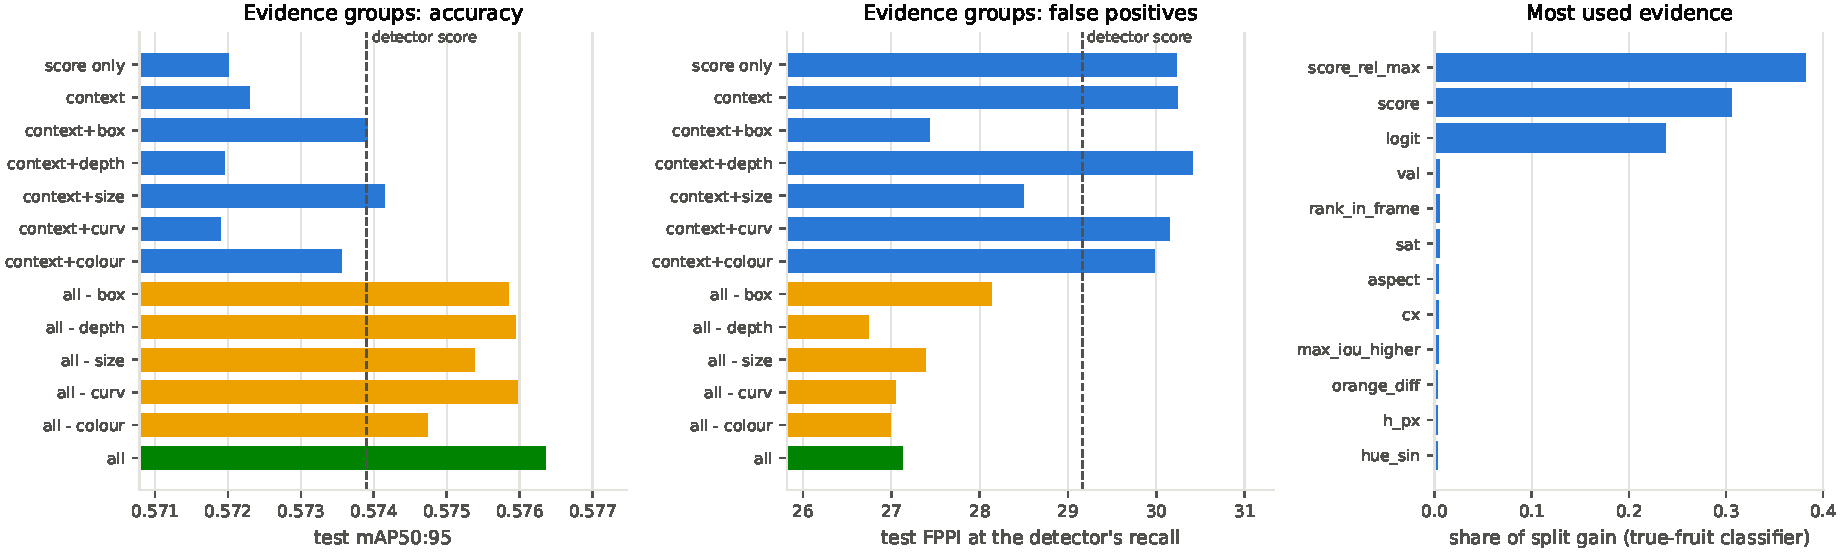
\includegraphics[width=0.98\linewidth]{../figures/fig_rescoring_ablation.pdf}
\caption{The complete evidence combination improves calibration results, while the classifier primarily uses detection confidence information. Panels show accuracy under feature-group ablation, false positives at the original recall, and feature importance in the true-fruit classifier.}
\label{fig:per}
\end{figure}
Figure~\ref{fig:per} explains evidence calibration through performance changes and feature usage. Relative scores, raw scores, and their logarithms account for most split gain, indicating that the calibrator builds its decisions around detection confidence. Complete evidence improves mAP50:95 and lowers false positives at matched recall relative to score-only calibration, demonstrating the practical value of additional candidate descriptors. Feature importance describes which evidence the model uses, while removal controls test how that evidence affects performance. Together, they support learning candidate quality after freezing the detector.

\subsection{Controlled Comparison with Geometric Detection Methods}
This section uses paired statistical analysis to examine differences between detection methods and geometric input conditions. Figure~\ref{fig:ladder} additionally shows performance increments due to input organization and output processing.

\begin{table}[H]
\centering
\scriptsize\setlength{\tabcolsep}{3pt}
\caption{Paired differences between detection methods and geometric input conditions. Held-out images are resampled 1,000 times; parentheses show 95\% intervals.}
\label{tab:geometry_stats}
\begin{adjustbox}{max width=\linewidth}
\begin{tabular}{>{\raggedright\arraybackslash}p{4.6cm}lllc}
\toprule
Comparison & $\Delta$ mAP50 & $\Delta$ mAP50:95 & \shortstack{$\Delta$ FPPI\\(confidence 0.25)} & $p$ \\
\midrule
Full-image RT-DETR-L $\rightarrow$ GeoSphere-DETR (common protocol) & $-$0.021 ($-$0.030 to $-$0.011) & $-$0.013 ($-$0.020 to $-$0.007) & $\mathbf{-29.7}$ ($-$30.9 to $-$28.5) & $<$0.001 \\




Full-image GeoSphere-DETR $\rightarrow$ \textbf{SOAD (complete)} & \textbf{+0.147} (+0.134 to +0.159) & \textbf{+0.157} (+0.148 to +0.165) & $-$16.1 ($-$16.9 to $-$15.4) & $<$0.001 \\
Tiled RGB $\rightarrow$ tiled GeoSphere-DETR (aligned geometry) & $-$0.009 ($-$0.018 to +0.000) & $-$0.003 ($-$0.009 to +0.004) & $-$21.7 ($-$22.5 to $-$20.9) & 0.472 \\
Same comparison, both with mirror fusion and rescoring & +0.002 ($-$0.005 to +0.009) & +0.004 ($-$0.001 to +0.009) & $-$0.4 ($-$0.5 to $-$0.2) & 0.100 \\
Tiled GeoSphere-DETR, before versus after loader alignment & $-$0.004 ($-$0.012 to +0.004) & +0.002 ($-$0.004 to +0.008) & $-$1.3 ($-$1.5 to $-$1.1) & 0.594 \\

Tiled GeoSphere-DETR, 640-pixel input versus 960-pixel fine-tuning & $-$0.006 ($-$0.016 to +0.003) & $-$0.010 ($-$0.018 to $-$0.003) & +1.5 (+1.2 to +1.7) & 0.002 \\
\bottomrule
\end{tabular}
\end{adjustbox}
\par\vspace{2pt}\parbox{0.97\linewidth}{\footnotesize $p$ denotes a two-sided bootstrap test for mAP50:95. FPPI differences involving rescoring compare different score scales at a fixed confidence threshold; comparisons at matched recall are given in Table~\ref{tab:main} and Fig.~\ref{fig:froc}. Bold marks the largest accuracy gain or false-positive reduction in each difference column; comparisons have different starting configurations.}
\end{table}
Table~\ref{tab:geometry_stats} verifies the benefit of complete SOAD against another full-image baseline. Relative to full-image GeoSphere-DETR, SOAD gains 0.157 mAP50:95, with a 95\% interval of 0.148--0.165 and $p<0.001$, providing statistical support for the combined effects of input organization and output processing. Under matched tiling, the geometric model's increments over the RGB model are $-0.003$ for single-view processing and $+0.004$ for complete processing. Both intervals include zero, illustrating how geometric gains depend on observation and processing conditions. This control implements the proposed framework for evaluating additional geometry under specified input conditions while separately quantifying overall pipeline gains and smaller differences between models.


\begin{figure}[H]
\centering
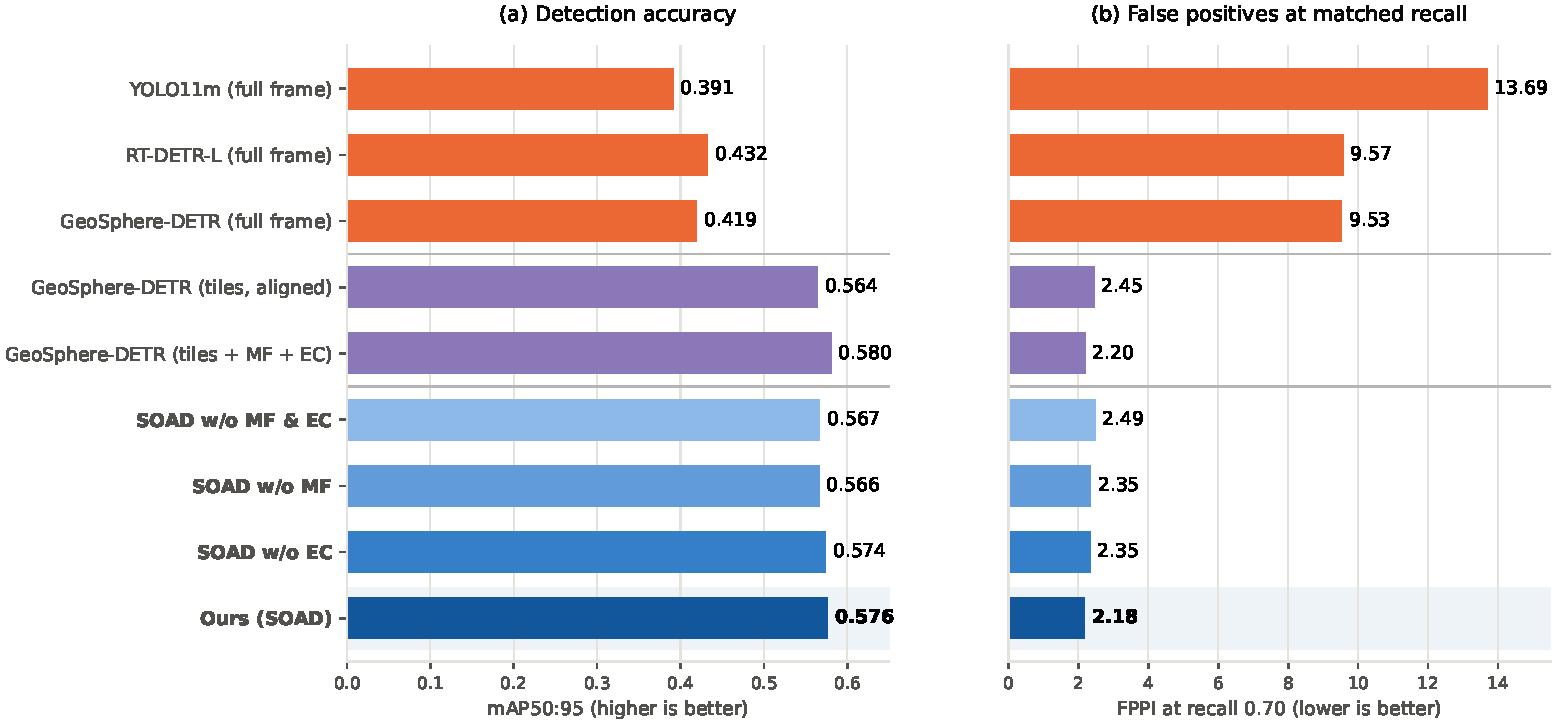
\includegraphics[width=0.98\linewidth]{../figures/fig_ladder.pdf}
\caption{Performance increments from SOAD input organization and output modules. Orange denotes full-image baselines, purple denotes geometric controls using aligned tiles, and blue denotes SOAD variants; complete SOAD appears in bold at the bottom. Left: mAP50:95. Right: false positives per image at recall 0.70. MF and EC denote mirror fusion and evidence calibration. All values are measured on the same held-out set.}
\label{fig:ladder}
\end{figure}
Figure~\ref{fig:ladder} shows how gains are distributed from local inputs to instance outputs in SOAD. Base SOAD gains 0.135 mAP50:95 over full-image RT-DETR-L, accounting for approximately 94\% of the complete pipeline's total gain of 0.144. FPPI@R.70 decreases from 9.57 to 2.49, indicating that tile training and instance aggregation provide the main performance contribution. Adding mirror fusion alone gives mAP50:95 of 0.574, whereas adding calibration alone gives 0.566; both have FPPI@R.70 of 2.35. The complete combination reaches 0.576 and 2.18, respectively. This result supports the functional roles of mirror fusion in improving detection accuracy and evidence calibration in refining candidate selection, and verifies their joint contribution to output quality.

The geometric tile control provides additional evidence for SOAD's false-positive control under matched processing. Complete geometric processing achieves mAP50:95 of 0.580, compared with 0.576 for SOAD, while their FPPI@R.70 values are 2.20 and 2.18, respectively. SOAD has fewer false positives at this operating point, providing supplementary evidence for background rejection. Figure~\ref{fig:ladder} shows the direction and magnitude of performance changes, while Tables~\ref{tab:ladder} and \ref{tab:geometry_stats} provide the corresponding statistical analyses.

\subsection{Computational Cost}

The scale comparison for the geometric model informs the choice of native 640-pixel tiles. The native configuration achieves test mAP50:95 of 0.564, exceeding the 0.554 obtained after resizing to 960 pixels and fine-tuning for four additional epochs. Directly increasing inference resolution on the validation set changes mAP50:95 from 0.626 to 0.545. For the tested geometric architecture and training conditions, this comparison supports retaining the native tile scale to achieve higher accuracy with a smaller input area.

Tiled inputs preserve more local pixels but increase the number of network executions. Figure~\ref{fig:cost} expresses computational cost as equivalent 640-pixel inference passes per image, scaling the 960-pixel configuration by input area. This metric excludes tile preparation, full-image deduplication, calibration feature extraction, and data transfer between devices.

\begin{figure}[H]
\centering
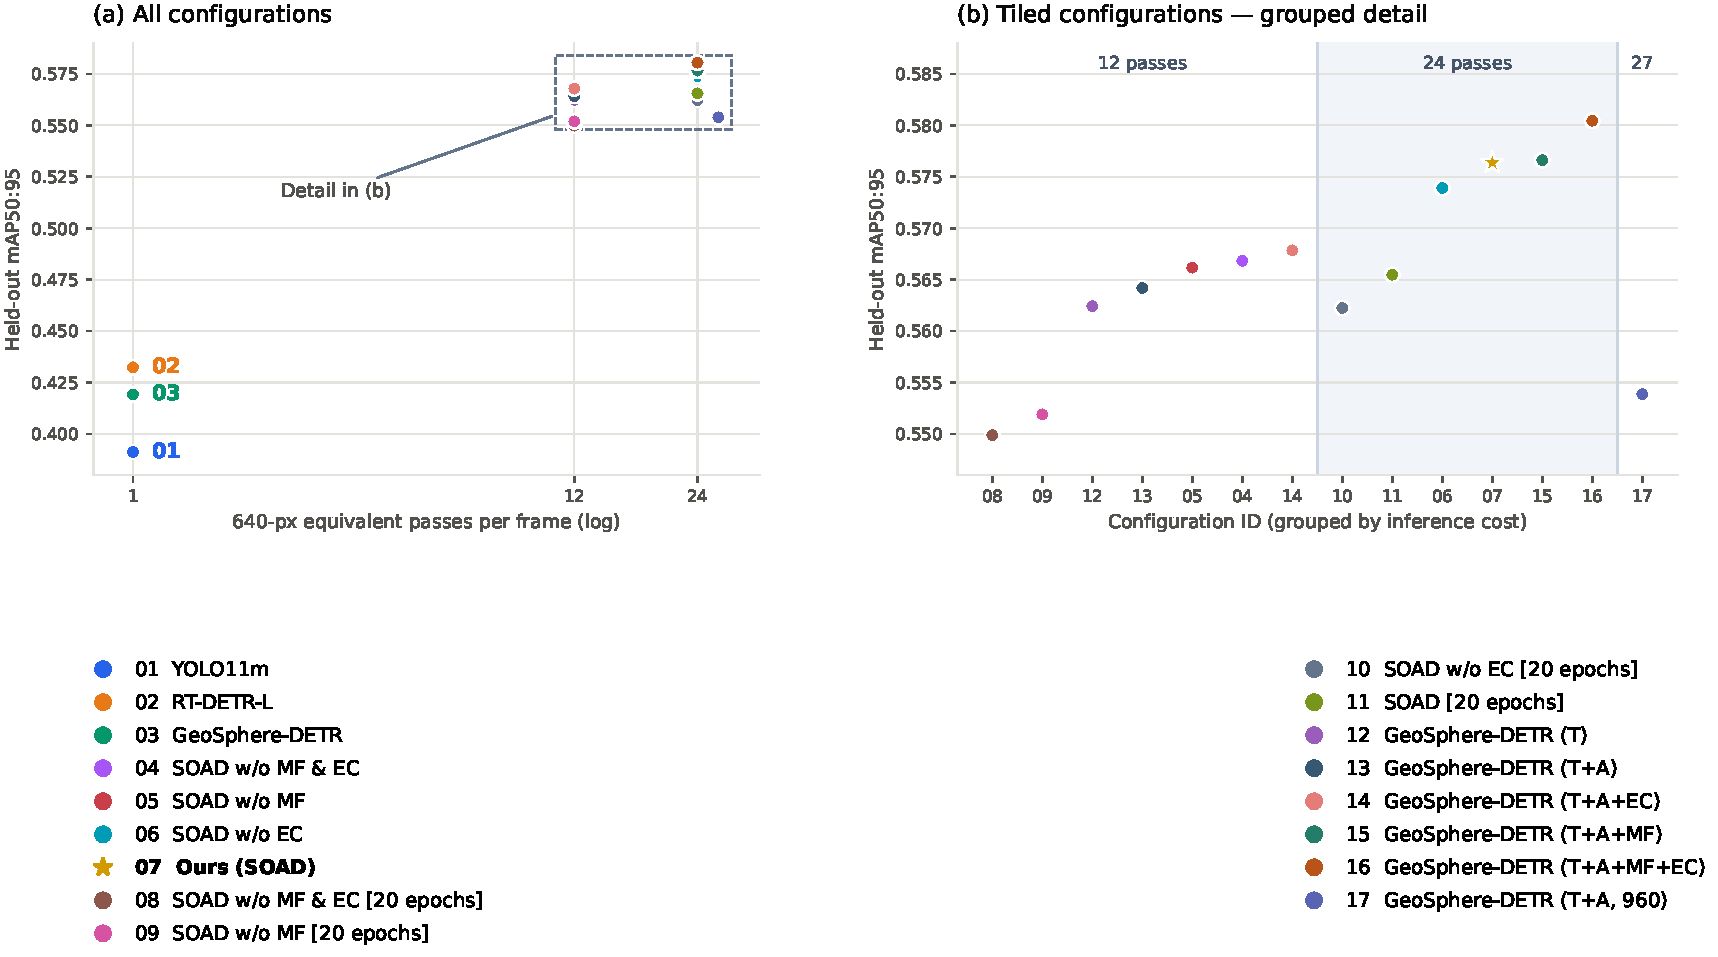
\includegraphics[width=0.98\linewidth]{../figures/fig_cost.pdf}
\caption{Detection accuracy versus inference cost. (a) All configurations. (b) Enlarged view of tiled configurations grouped by inference cost, with configuration identifiers on the horizontal axis. Each configuration has a distinct color, identifiers correspond to the legend below, and stars indicate complete SOAD. MF, EC, T, and A denote mirror fusion, evidence calibration, tiled input, and synchronized alignment, respectively. The 640-pixel configurations are measured by network pass counts, while the 960-pixel configuration is converted to 27 equivalent passes based on input area. Calibration and data processing time are excluded.}
\label{fig:cost}
\end{figure}
Figure~\ref{fig:cost} shows that SOAD's base input pipeline provides most of the accuracy gain. The base configuration performs twelve tile inference passes and achieves mAP50:95 of 0.567, compared with 0.576 for the complete configuration. It accounts for approximately 94\% of the improvement over the full-image baseline of 0.432. Mirror fusion further improves accuracy, establishing a progression in which input organization provides the main increase and output fusion adds further refinement. These results support SOAD's modular design in terms of both accuracy and inference cost. Computation is measured using network calls and input-area conversion; end-to-end latency is a separate deployment metric.
All models are trained with a single random seed. Paired bootstrap intervals quantify test-image sampling variation with model weights fixed. The dataset covers citrus fruits and the sensors used for its acquisition; cross-orchard testing evaluates scene transfer under these acquisition conditions. The calibrators are fitted using 200 validation images from the training orchard. Their transfer across orchards is evaluated through detection ranking, false positives at matched recall, and counting error. The roles of depth and curvature features are assessed by the removal controls in Table~\ref{tab:per}.

\section{Conclusion}
We presented SOAD, a complete detection pipeline integrating training on native-pixel tiles, cross-tile instance aggregation, mirror fusion, and evidence calibration. Under comparable training iteration budgets, the base pipeline improves held-out orchard mAP50:95 from 0.432 for the full-image RGB baseline to 0.567, and the complete configuration reaches 0.576. At recall 0.70, FPPI decreases from 9.57 to 2.18. Paired tests support a significant accuracy gain over the full-image baseline, while component ablations further verify the complementary roles of mirror fusion and evidence calibration in accuracy and counting. The geometric control with matched processing achieves mAP50:95 of 0.580, whereas SOAD has fewer false positives at matched recall. Together, the experiments support organizing dense citrus detection from input observations through instance aggregation to candidate quality estimation. The measured gains pertain to the complete pipeline, which jointly adjusts object scale, context, and sample composition.

\section*{Data and Code}
The dataset is available from \cite{dataset}. Numerical results, detections, analysis scripts, and original figure files are provided in the accompanying project directory. Figure labels, captions, and the manuscript text are presented in English.

\begin{thebibliography}{99}\small
\bibitem{rtdetr} Y. Zhao et al., “DETRs Beat YOLOs on Real-time Object Detection,” \emph{Proc. IEEE/CVF CVPR}, 2024, pp. 16965--16974. \url{https://arxiv.org/abs/2304.08069}
\bibitem{rtdetrv2} W. Lv et al., “RT-DETRv2: Improved Baseline with Bag-of-Freebies for Real-Time Detection Transformer,” arXiv:2407.17140, 2024. \url{https://arxiv.org/abs/2407.17140}
\bibitem{agyolo} Y. Lin et al., “AG-YOLO: A Rapid Citrus Fruit Detection Algorithm with Global Context Fusion,” \emph{Agriculture}, vol. 14, no. 1, 114, 2024. doi:10.3390/agriculture14010114.
\bibitem{mfaf} Y. Zhang et al., “Multi-scale feature adaptive fusion model for real-time detection in complex citrus orchard environments,” \emph{Computers and Electronics in Agriculture}, vol. 219, 108836, 2024. doi:10.1016/j.compag.2024.108836.
\bibitem{yuyolo} Y. Yu et al., “Object Detection Algorithm for Citrus Fruits Based on Improved YOLOv5 Model,” \emph{Agriculture}, vol. 14, no. 10, 1798, 2024. doi:10.3390/agriculture14101798.
\bibitem{geosphere} S. Liu et al., “GeoSphere-DETR: RGB-D citrus fruit detection in cluttered orchards via geometry-gated fusion and geometry-aware confidence recalibration,” \emph{Artificial Intelligence in Agriculture}, 2026. doi:10.1016/j.aiia.2026.08.010.
\bibitem{sahi} F. C. Akyon, S. O. Altinuc, and A. Temizel, “Slicing Aided Hyper Inference and Fine-tuning for Small Object Detection,” \emph{Proc. IEEE ICIP}, 2022, pp. 966--970. doi:10.1109/ICIP46576.2022.9897990.
\bibitem{asahi} F. Moretti, Y. Jin, and G. Mario, “Adaptive Slicing-Assisted Hyper Inference for Enhanced Small Object Detection in High-Resolution Imagery,” arXiv preprint arXiv:2604.19233, 2026. \url{https://arxiv.org/abs/2604.19233}
\bibitem{ciafnet} Y. Chen et al., “CIAFNet: An RGB-D Cross-Modal Interaction and Adaptive Fusion Network for Camellia oleifera Fruit Detection,” \emph{Agriculture}, vol. 16, no. 17, 1884, 2026. doi:10.3390/agriculture16171884.
\bibitem{bpc} M. A. Munir et al., “Bridging Precision and Confidence: A Train-Time Loss for Calibrating Object Detection,” arXiv:2303.14404, 2023. \url{https://arxiv.org/abs/2303.14404}
\bibitem{dataset} Citrus fruit RGB-D data set, Hugging Face, CC BY 4.0. \url{https://huggingface.co/datasets/ariel0818/citrus-fruit-rgbd}
\bibitem{wbf} R. Solovyev, W. Wang, and T. Gabruseva, “Weighted boxes fusion: ensembling boxes from different object detection models,” \emph{Image and Vision Computing}, vol. 107, 104117, 2021.
\bibitem{lgbm} G. Ke et al., “LightGBM: A Highly Efficient Gradient Boosting Decision Tree,” \emph{Advances in Neural Information Processing Systems}, vol. 30, 2017.
\bibitem{yolo11} Ultralytics, “Ultralytics YOLO11,” official model documentation, released September 27, 2024. \url{https://docs.ultralytics.com/models/yolo11/}
\bibitem{yolov10} A. Wang et al., “YOLOv10: Real-Time End-to-End Object Detection,” \emph{Advances in Neural Information Processing Systems}, vol. 37, 2024. \url{https://arxiv.org/abs/2405.14458}
\bibitem{dfine} Y. Peng et al., “D-FINE: Redefine Regression Task of DETRs as Fine-grained Distribution Refinement,” \emph{Proc. ICLR}, 2025. \url{https://arxiv.org/abs/2410.13842}
\bibitem{deim} S. Huang et al., “DEIM: DETR with Improved Matching for Fast Convergence,” \emph{Proc. IEEE/CVF CVPR}, 2025, pp. 15162--15171. \url{https://openaccess.thecvf.com/content/CVPR2025/html/Huang_DEIM_DETR_with_Improved_Matching_for_Fast_Convergence_CVPR_2025_paper.html}
\bibitem{mecd} Y. Liao et al., “YOLO-MECD: Citrus Detection Algorithm Based on YOLOv11,” \emph{Agronomy}, vol. 15, no. 3, 687, 2025. doi:10.3390/agronomy15030687.
\bibitem{acdnet} Z. Wang, W. Xia, and M. Li, “ACDNet: Adaptive Citrus Detection Network Based on Improved YOLOv8 for Robotic Harvesting,” \emph{Agriculture}, vol. 16, no. 2, 148, 2026. doi:10.3390/agriculture16020148.
\bibitem{scoredetr} B. Zhang et al., “SCORE-DETR: An efficient Transformer-based network for small and occluded citrus detection,” \emph{Computers and Electronics in Agriculture}, vol. 238, 110843, 2025. doi:10.1016/j.compag.2025.110843.
\bibitem{fgdetr} Y. Wei et al., “Fine-grained multi-scale feature fusion for robust citrus detection under complex orchard conditions,” \emph{Applied Soft Computing}, vol. 201, 115506, 2026. doi:10.1016/j.asoc.2026.115506.
\bibitem{trackcal} D. Lee, J. Lee, J. Lee, and J. Choi, “Annotation-free confidence calibration of object detectors via object tracking,” \emph{Pattern Recognition Letters}, vol. 209, pp. 194--201, 2026. doi:10.1016/j.patrec.2026.09.016.
\end{thebibliography}
\end{document}
